% !TEX root = ../thesis_main.tex
%
%
%
%%%% --- * --- %%%%	
%\clearpage
%\chapter{Introduction}
\chapter{Background}
\label{intro_chapter}
\label{nuclear_chapter}
Within nature, there exist four fundamental forces governing the interactions of particles with one another:  electromagnetism, the nuclear weak force, the nuclear strong force, and gravity.  This work seeks to probe the nature of the weak nuclear force on its most fundamental level through observations of beta decay, a process which results directly from the action of the weak nuclear force.  Through kinematic observations of the decay products, much can be learned about the form of the weak nuclear force's coupling, through which beta decay proceeds.  Prior experiments have shown that this coupling is dominated by a combination of so-called vector and axial couplings, but the possibility of a non-dominant contribution from other types of operators, such as scalars and tensors, cannot be ruled out entirely.  This is the domain of precision measurements.  

\section{Introduction}
\label{section:intro}
\note{...on the Four Forces}
% 4 forces
Within our present understanding of physics, there are four fundamental forces governing the interactions of particles with one another:  electromagnetism, the nuclear weak force, the nuclear strong force, and gravity.  These forces are considered to be distinct from one another by virtue of their differing behaviours, however attempting to unify them within a single theoretical framework has been a major focus of later 20th- and early 21st century physics to date.  The effort has been met with only partial success, and the resulting theoretical framework is collectively known as the \ac{SM}.

% Standard Model
The standard model provides a quantum mechanical description for
%which includes quantitative models of 
the behaviour of three of the four fundamental forces:  electromagnetism, the nuclear weak force, and the nuclear strong force.  The \ac{SM} notably does not describe gravitational processes --- despite extensive efforts, the gravitational force has thus far defied all attempts to describe it in a fully quantum mechanical way, though this remains an active field of research.  

%
Each force has its own specific mediating particle(s) which couple only to a particular type of (generalized) charge, and therefore interact only with particles that possess that charge.  For example, the gravitational charge is \emph{mass}, and (at least within a simplified particle physics model) gravity acts only on objects that possess mass.~\aside{Can I turn this into a footnote?  It's not true because the curvature of spacetime also affects photon trajectories, and there even exist (unstable) (quasi-?) bound states comprised *only* of photons, as in e.g. Aichelburg-Sexl.}  With only a single type of charge and no negative masses, the gravitational force can only ever be attractive.
%
By constrast, the electromagnetic force couples to both positive and negative electric charges, and can produce both attractive and repulsive forces.  Both the electromagnetic and gravitational forces are mediated by massless force-carrying particles (the photon and still-theoretical graviton, respectively), a property which implies that the amount of flux per unit solid angle is constant over all distance scales, and Gauss's Law holds true.
% allows them to act even over long distances, as it implies that the amount of flux per unit solid angle is constant over all distance scales, leading to, e.g., the applicability of the famous Gauss's Law.  \aside{cite someone for Gauss's Law.}

\begin{figure}[h!t!b!]
	\centering
	\includegraphics[width=.80\linewidth]{Figures/feynmandiagrams_general_placeholdercropped.pdf}
	\note[tag]{Fix Feynman vertex placeholder figure.}
	\caption[An exhaustive list of weak vertices]{An exhaustive list of weak vertices.  All possible Feynman diagram vertices involving $W^+$, $W^-$, or $Z^0$ bosons are shown.  Time goes up.  The usual rules for Feynman diagram vertices apply.}	
	\label{fig:feynmandiagrams_general}
\end{figure}

In the case of the nuclear weak force, which will be the primary concern within this thesis, 
the notion of generalized charge is no longer entirely straightforward to apply.
%, which could be readily applied to the gravitational and electromagnetic forces, is no longer entirely straightforward to apply.  
We must rely instead on a list of allowed Feynman diagram vertices to describe the types of interaction that are possible (see Fig.~\ref{fig:feynmandiagrams_general}).  We note that the weak force involves three mediating particles --- $W^+$, $W^-$, and $Z^0$ bosons --- and these mediators can interact with both (anti-)quarks and (anti-)leptons.  The $W^+$ and $W^-$ particles also carry electric charge, which must be separately conserved in any interaction,~\aside{(wait, is that true?  what about with the photon vertex? ....I think it's fine.....} but the $Z^0$ is electrically neutral.  All three are massive, which implies that the strength of the weak force falls off more rapidly as distance increases, and Gauss's Law does not apply. 

%Despite the large number of possible weak force interaction vertices, 
%develop an intuition about the types of interactions that are possible (see Fig.~\ref{fig:feynmandiagrams_general}).  
%%%%\begin{figure}[h!tb]
%%%%	\centering
%%%%	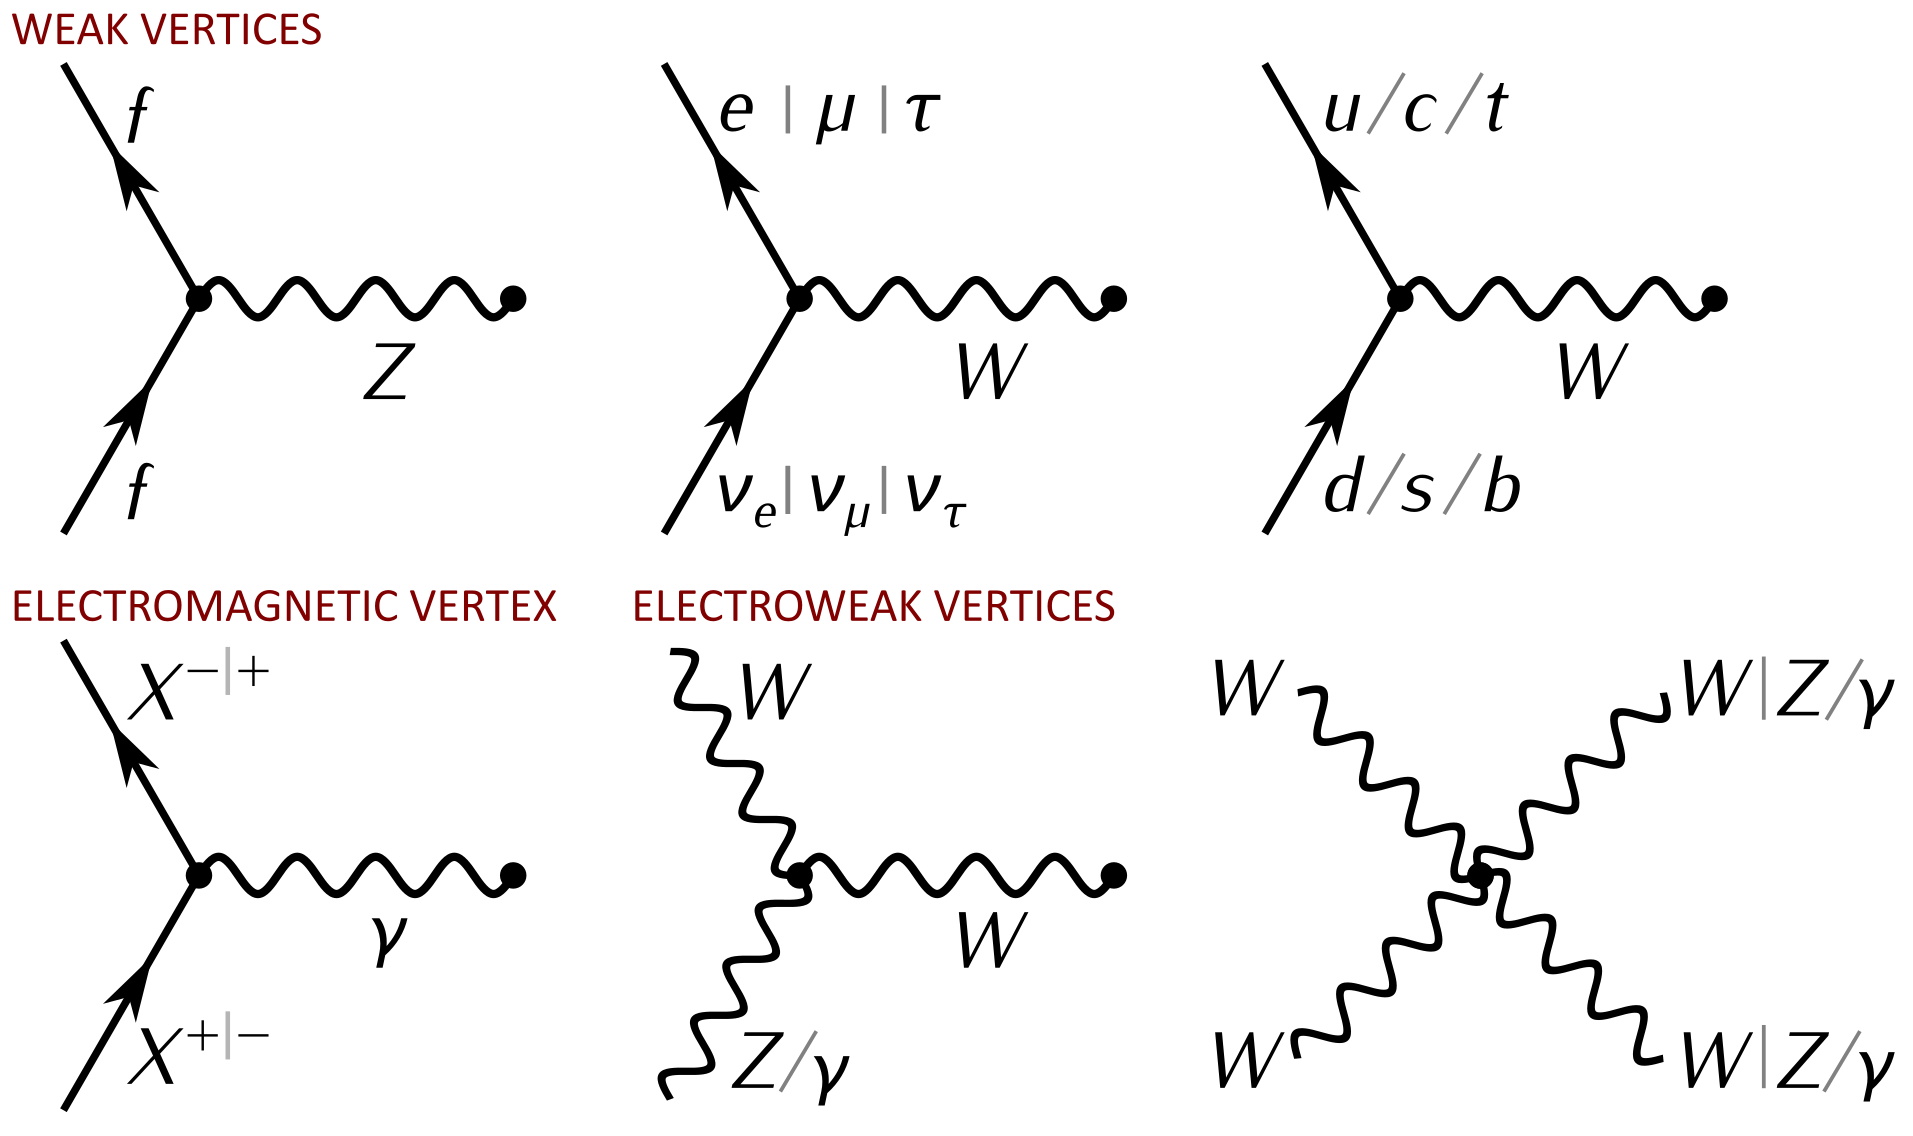
\includegraphics[width=.999\linewidth]{Figures/feynmanvertices_placeholder.png}
%%%%	\note{I have to re-make this figure.  This one doesn't belong to me.  Also, I'm not necessarily sure I believe/understand what it's saying on the bottom line.}
%%%%	\caption[Allowed Weak Vertices]{Allowed Weak Vertices:  a placeholder figure.  Top left:  $f$ is any fermion.  Top centre:  Lepton flavour is conserved under the weak interaction.  Top right:  quark generation is not conserved under the weak interaction.}	
%%%%	\label{fig:feynmandiagrams}
%%%%\end{figure}



With a comparatively large number of possible vertex types, it can be challenging to develop an intuition about the behaviour of the weak force. 
%and the vertices involving only gauge bosons are especially inscrutable.
%Arguably the most well-known result of the weak force is radioactive beta decay, 
Perhaps the most well known physical behaviour that arises from the nuclear weak force is beta decay. 
% (Fig.~\ref{fig:feynmandiagrams_betadecay}).  
In Fig.~\ref{fig:feynmandiagrams_betadecay} the tree-level Feynman diagrams pertaining to the most common beta decay processes are shown.  It is these beta decay processes which present what is arguably the most accessible experimental window on the workings of the nuclear weak force.


\FloatBarrier
\begin{figure}[h!t!b!]
	\centering
	\includegraphics[width=.90\linewidth]{Figures/feynmandiagrams_betadecay_placeholder.jpeg}
	\note[tag]{Fix beta decay Feynman diagram placeholder figure.}
	\caption[Beta Decay Feynman Diagrams]{Beta decay Feynman diagrams are shown here at the nucleon(? sort of) level.    
	}	
	\label{fig:feynmandiagrams_betadecay}
\end{figure}


%The nuclear weak force is one of four fundamental forces described within physics.  
%It mediates the process of beta decay, which is of particular interest to us here.  
Although beta decay is generally well understood, it presents a unique opportunity for precision measurements to search for physics beyond the Standard Model within the weak coupling.
By observing the kinematics and angular correlations involved in the decay process, one gains access to a wealth of information about the form of the operators mediating the decay.  

\aside{Something something ... it's so well understood that all that's left to do is the precision measurements.}

%\note[jbn]{Standard Model -> standard model of particle physics (often denoted here "SM"). 
%\\
%The standard model is ...
%\\...\\
%Weak -> weak.
%\\...\\
%This of course is the place where Georg wants more for orientation.
%}


%Attempting to unify the four fundamental forces within a single theoretical framework has been a major focus of later 20th- and early 21st century physics to date, however the effort has thus far been met with only partial success.

\note[orange, nolist]{
\begin{itemize}
	\item (we're not proposing a new feynman diagram.  Just, a new vertex factor thingy, I guess.)
	\item Weak force lagrangian!  I think possibly it's only for the *charged* weak force??
	\item ...then we demand that the Lagrangian must be Lorentz invariant, otherwise we break physics.
%	\item weak force moderated by massive particles -- so it can't be as long range, and Gauss's Law doesn't hold.
	\item within this thesis, we will focus primarily on the \emph{charged} weak interactions (using $W^{\pm}$ as mediators rather than $Z^0$), with first-generation normal matter quarks (\emph{i.e.} up ($u$) and down ($d$) quarks, but not charm ($c$), strange ($s$), top ($t$), or bottom ($b$) quarks; no anti-quarks ($\bar{q}$ for $q=\{u,d,c,s,t,b \}$ )) and first-generation leptons (\emph{i.e.} electrons, positrons, electron neutrinos and electron anti-neutrinos, but not positive or negative muons or taus, nor muon or tau neutrinos or anti-neutrinos).
	\item Really, we'll only be looking at weak force interactions involving the two most common nucleons -- protons and neutrons.  ...each of which is a (meta-)stable bound state involving three quarks.  
%	\item the weak force couples to both leptons and quarks.
	\item masses of W and Z bosons?  
%	\item graviton -- theoretical only.
%	\item strong force -- beyond the scope.
\end{itemize}
}


%%%%%Within the present understanding of physics, there are four fundamental forces governing the interactions of particles with one another:  electromagnetism, the nuclear weak force, the nuclear strong force, and gravity. 
%%%%%%
%%%%%Among other things, these four forces are considered distinct by virtue of the fact that each one couples to a different type of charge and is mediated by a different type of particle.  The result is that each force has potentially different behaviour at varying length scales.  
%%%%%%
%%%%%The most familiar example of this is a comparison between the forces of electromagnetism and gravity.  While the electromagnetic force couples to both positive and negative electric charges, and can therefore create both attractive and repulsive forces, the gravitational force couples only to (positive) mass, and the result is a force that is only attractive and never repulsive.  Both forces are mediated by massless particles (the photon and graviton, respectively), which implies that the strength of the two forces must fall off at the same rate as the distance between interacting bodies is increased.  In the case of the nuclear weak force, the mediator particles are massive, ...
%%%%%
%%%%%Attempting to unify the four forces within a single theoretical framework has been a major focus of later 20th- and early 21st century physics to date, however the effort has thus far been met with some limited success.


%Attempts to unify the four forces within a single model have been a major focus of 20th- and 21st century physics, }

%%%Both are mediated by massless particles (the photon and graviton, respectively)
%%%Because these are both mediated by massless particles (the photon and graviton, respectively), their behaviour 



%%%% --- * --- %%%%	
%\section{An Abbreviated Look at the History of Beta Decay}
\section{A Historical Look at Beta Decay and the Weak Interaction}
%\note[tag]{History section needs *all* the citations.}

We consider the historical development of our scientific understanding of beta decay and the nuclear weak force.  This is a historically rich topic, and a full discussion is beyond the scope of this document, however we shall attempt to touch on some highlights.

Radioactivity was first observed in 1896 by Henri Becquerel in uranium, and this landmark discovery set off a flurry of activity in the field~\cite{becquerel1896}.
% With our modern understanding of radioactive decay, we know that this of course could not have been beta decay, but rather a combination of alpha decay and spontaneous fission -- however it was this observation that set the field into motion.  
Ernest Rutherford noted in 1899 that the particles emitted by a sample of uranium could be classified into two groups based on how readily they were absorbed in materials -- alpha particles are easily absorbed, while beta particles are more penetrating~\cite{rutherford1899}.  A third and even more penetrating type of radioactive emission was observed in 1900 by Paul Villard, who made no attempt to give it a name -- but within a few years, Rutherford's naming convention had been applied and this third type of particle became known as a gamma ray~\cite{villard1900}\cite{rutherford1903}.  

\note{Rutherford discovered that:  half-life.  [76]=E. Rutherford, \emph{Phil. Mag.} \textbf{49}, 1, 1900.  Thorium.  Rn220.  ...but also, *I* got this from Abraham Pais.}

When, in 1900, Becquerel measured the charge-to-mass ratio of emitted beta ($\beta^-$) radiation and found that it was the same as that of the electron, he proposed that these must be the same particle~\cite{becquerel1900},~\aside{I think.  Also, I think that's the right citation..} and in 1903~\aside{or possibly 1901?} Rutherford and Soddy demonstrated that the processes of alpha and beta decay both transmute the original chemical element into another\cite{rutherfordsoddy1903}.
\aside{That arxiv rando claims that the half-life thing was developed or hinted at by 1900 Rutherford, but who the fuck knows?}

Despite these early successes, in 1911 Lise Meitner and Otto Hahn noticed that beta particles are emitted with a variety of different kinetic energies,~\aside[tag]{citation needed} and in 1914 James Chadwick
%%~\aside{citation needed.  also, maybe it was a bunch of people, 1914-1927.  
%%\\
%%Chadwick's original:  Chadwick, J. (1914). "Intensitätsverteilung im magnetischen Spektren der β-Strahlen von Radium B + C". Verhandlungen der Deutschen Physikalischen Gesellschaft (in German). 16: 383–391.  
%%\\
%%Maybe also Charles Drummond Ellis?  
%%\\
%%Ellis and Wooster:  Ellis, C. D.; Wooster, W. A. (1927). "The Continuous Spectrum of β-Rays". Nature. 119 (2998): 563–564. doi:10.1038/119563c0. S2CID 4097830.  } 
demonstrated that energies of emitted beta particles formed a continuous distribution.  The physics community was baffled for years by the fact that it seemed impossible to predict the energy of a beta particle emitted by a particular process;  if the emitted beta simply took on the difference in energy between the initial and final states, then surely that energy should be a fixed, unchanging value for a paricular transition. 

%should be a fixed amount of energy for a given transition.  
Finally, in 1930, a frustrated Wolfgang Pauli famously proposed that if an additional small, neutral, difficult to detect particle were emitted simultaneously with the beta and allowed to carry away a varying amount of energy, then this accounting trick could account for the continuous beta energy spectrum.
%could account for the continuous beta energy spectrum, by carrying away whatever fraction of the
%This new particle was dubbed a ``neutron'' 
He named this particle a ``neutron'' -- though today we refer to that same particle as a(n) ``(anti-)neutrino,'' and use the name ``neutron'' for an entirely different particle\cite{PauliNeutrino1978}.  \aside{Fermi renamed it, because Italian.}

%When Enrico Fermi offered a quantitative description of 
Pauli's 1930 insight paved the way for Enrico Fermi to propose a quantitative description of the nuclear weak force and the beta decay processes resulting from it.  He modeled the weak force as a contact interaction with zero range --- a very good approximation.  After being rejected by \emph{Nature} in 1933, Fermi's seminal theory of beta decay was published in both Italian and German journals the following year \cite{AbrahamPais} \cite{Fermi1934Italian} \cite{Fermi1934German}.
%\aside[done]{Citation is:  Pais, Abraham (1986). Inward Bound. Oxford: Oxford University Press. p. 418. ISBN 0-19-851997-4. \cite{AbrahamPais} }  
Because of its powerful predictive ability together with its generalized quantum mechanical approach, Fermi's model forms the basis upon which modern beta decay calculations have been built.  With one of its major results, now commonly known as Fermi's Golden Rule, still routinely used, the introduction of Fermi's model arguably marks the beginning of our modern understanding of beta decay.

%%
%%its introduction arguably marks the beginning of our modern understanding of the topic. 
%%With one of its major results, now commonly known as Fermi's Golden Rule, still routinely taught 

%With one of its major results --- now commonly known as Fermi's Golden Rule --- still applicable for many modern calculations~\aside{rephrase} due to its powerful predictive ability together with its generalized quantum mechanical approach to the problem, Fermi's model arguably marks the beginning of our modern understanding of beta decay (see Sec.~\ref{}).

%%%\note[done]{Pauli and the neutrino:  
%%%\\...\\
%%%Brown, L.M. (1978). "The idea of the neutrino". Physics Today. 31 (9): 23–28. Bibcode:1978PhT....31i..23B. doi:10.1063/1.2995181.~\cite{PauliNeutrino1978}}

%The introduction of Fermi's theory of beta decay arguably marks the beginning of our modern understanding of the field.  
%Now commonly known as Fermi's Golden Rule, 
%One of the major results in this is now commonly known as Fermi's Golden Rule,  

%Now known as Fermi's Golden Rule, the introduction of this model
%arguably marks the beginning of our modern understanding of beta decay.  Fermi's Golden Rule is both remarkably general in its approach and powerful in its predictive power, approaching the matter from a fully quantum mechanical perspective (see Section~\ref{}).~\aside{add link} 

%On the experimental front,~\aside{Rephrase.} 
The mid 1930s was a busy time 
%1934 was a busy year 
for our understanding of beta decay.  In addition to the publication of Fermi's model in 1934, this year also marks the first discovery of $\beta^+$ radiation, for which Irène and Frédéric Joliot-Curie later received a Nobel prize, and the proposal by Gian-Carlo Wick of the electron capture mechanism for beta decay.  
%This was also the year when the electron capture mechanism for beta decay was first proposed by Gian-Carlo Wick.  
The electron capture theory was fleshed out further in 1935-1936 by Yukawa and Sakata\aside{and others?},\aside{Yukawa and Sakata first names?} and first observed in 1937 by Luis Alvarez.  Meanwhile, in 1936 George Gamow and Edward Teller improved upon Fermi's model by including a mechanism to potentially change the nuclear spin\cite{GamowTeller}, and to this day, beta decay transitions are still routinely classified as following Fermi or Gamow-Teller (or mixed) selection rules.

%~\aside{omg, I can't just give first names for only the non-Asian people...}
%\note[tag]{Gamow-Teller in 1936\cite{GamowTeller}. }
%1934 was also the year when Wick proposed the electron capture mechanism for beta decay, later observed by Luis Alvarez in 1937.  \aside{Yukawa and others totes helped flesh out the theory behind E.C.  Or possibly they proposed it first?  who even knows.}
Over the next few years, developments within the field of nuclear physics were largely directed elsewhere, but beta decay returned to scientific prominence with T. D. Lee and C. N. Yang's 1956 suggestion~\aside[tag]{Probably point out that this thing is the basis for the model of the weird-ass currents I'm looking for.  They made a (nucleon-level) Hamiltonian with *everything*.} 
that, contrary to the community's prior expectation, parity may not be conserved within beta decay processes\cite{LeeYang}.
~\aside{their hamiltonian operates at the nucleon level, because they hadn't discovered quarks yet.  also, this is the basis for where we're going with this experiment.  shows all possible Lorentz-invariant contributions to the thingy. V,A,S,T,P.  I don't think they knew about W and Z bosons either.}  The proposition was rapidly put to the test by C.S. Wu's landmark 1957 measurement of $^{60}$Co, confirming that beta decay violates parity conservation and simultaneously paving the way for the Nobel prize to be awarded to Lee and Yang that same year~\cite{wu}.~\aside{nobel prize citation?}
~\aside{For a while everyone thought it was S,T.  But it turns out it's V,A.  Ben cites these guys for S,T:  \cite{RustadRuby1955tensor}\cite{BurgyEpstein1957scalartensor}.  though, the one article is before Wu. Also, I can't access these things.  Look at JTW's refs maybe..}
%\note{... a discovery which earned Lee and Yang a Nobel prize.  Wu's discovery earned Lee and Yang the 1957 Nobel Prize.}

Subsequent experiments demonstrated that not only was parity non-conserved in a beta decay transition, it is (as near as we can collectively tell) \emph{maximally} violated.  \aside{cite someone for maximal parity violation.}
Though it was initially believed that the couplings were comprised of so-called scalar and tensor interactions,\aside{cite someone for S,T !} Feynman and Gell-Mann first postulated the correct $(V-A)$ form of the interaction in 1958 by invoking an analogy with the photon, and this was eventually borne out by experimental evidence\cite{FeynmanGellMann1958}.  (See Sec.~\ref{sec:modernprecision} for further discussion on the form of weak interaction couplings.)
\aside{cite someone for $(V-A)$ evidence}
%it was subsequently determined 
%\note{Feynman and Gell-Mann postulated the $V-A$ form of the interaction in 1958, by analogy with the E\&M photon\cite{FeynmanGellMann1958}.  }

%\note{}
%We must now backtrack slightly to account for modern theoretical development relating to beta decay.  
%describe the theoretical development that 
%Many of the subsequent developments in the field came 
In the following years, the theory behind the nuclear weak force was developed further, and eventually merged with the theory of electromagnetism as the electroweak force.  The framework for \ac{QED} had already been largely developed between 1946 and 1950 by Shinichiro Tomonaga, Julian Schwinger, Richard Feynman, and others.  The theory was fully covariant, meaning that it behaves properly under a Lorentz transformation.  The work of Schwinger, and independently, Tomonaga, developed much of the methodology behind renormalization, which is now considered to be a mathematical necessity in any modern quantum field theory\cite{tomonaga1946}\cite{schwinger1948covariant}\cite{feynman1949spacetime}\cite{feynman1949positrons}\cite{feynman1950}\cite{dyson1949theories}.  ~\aside{QED as a "template" for other theories.}

%%%\note[done]{References for first sentence:
%%%\\ ... \\
%%%S. Tomonaga (1946). "On a Relativistically Invariant Formulation of the Quantum Theory of Wave Fields". Progress of Theoretical Physics. 1 (2): 27–42. doi:10.1143/PTP.1.27. \cite{tomonaga1946}
%%%\\
%%%J. Schwinger (1948). "On Quantum-Electrodynamics and the Magnetic Moment of the Electron". Physical Review. 73 (4): 416–17. doi:10.1103/PhysRev.73.416. \cite{schwinger1948magnetic}  (Really?  Do I really want to cite this thing, given the other thing? ... no, I don't think so.)
%%%\\
%%%J. Schwinger (1948). "Quantum Electrodynamics. I. A Covariant Formulation". Physical Review. 74 (10): 1439–61. doi:10.1103/PhysRev.74.1439.,  \cite{schwinger1948covariant}
%%%\\
%%%R. P. Feynman (1949). "Space–Time Approach to Quantum Electrodynamics". Physical Review. 76 (6): 769–89. doi:10.1103/PhysRev.76.769., \cite{feynman1949spacetime}  (Yeah, I think this is relevant.)
%%%\\
%%%R. P. Feynman (1949). "The Theory of Positrons". Physical Review. 76 (6): 749–59. doi:10.1103/PhysRev.76.749., \cite{feynman1949positrons}  (Possibly less relevant?)
%%%\\
%%%R. P. Feynman (1950). "Mathematical Formulation of the Quantum Theory of Electromagnetic Interaction" (PDF). Physical Review. 80 (3): 440–57.  doi:10.1103/PhysRev.80.440.,  \cite{feynman1950}
%%%\\
%%%F. Dyson (1949). "The Radiation Theories of Tomonaga, Schwinger, and Feynman". Physical Review. 75 (3): 486–502. doi:10.1103/PhysRev.75.486., \cite{dyson1949theories}
%%%\\ ... \\
%%%Also, do I maybe want to look at Dyson's thing that might actually be more relevant?  \cite{dyson1949Smatrix}.  Nope.  I don't think so.  Maybe I don't want to mention him by name at all.
%%%}

\note{From Wikipedia:  ``In 1957, Robert Marshak and George Sudarshan and, somewhat later, Richard Feynman and Murray Gell-Mann proposed a $V-A$ Lagrangian for weak interactions.''
\\...\\
``In the Standard Model, the $W^\pm$ and $Z^0$ bosons, and the photon, are produced through the spontaneous symmetry breaking of the electroweak symmetry SU(2) × U(1)Y to U(1)em, ...''
}

Following the success of QED, there was a push from the physics community to create a similar theory to model the nuclear weak force.  In 1961, Sheldon Glashow extended some of Schwinger's work to model the nuclear weak force,  adding an explicit mass term (i.e., to make the force mediating particles massive).  The model included the $W^+$ and $W^-$ bosons needed to explain beta decay, and for the first time, a neutral $Z^0$ boson.  With the explicit mass term, the theory was not renormalizable, and since there had been no experimental hint of the $Z^0$, Glashow himself discounted the model, and it initially received little attention.  In 1964, Abdus Salam and John Clive Ward proposed a similar theory, this time including the photon as well as $W^\pm$ and $Z^0$ bosons -- however they, too, relied on explicit symmetry breaking to provide a mass for the $W^\pm$ and $Z^0$ bosons\cite{Glashow1959}\cite{Glashow1961}\cite{SalamWard1964}.
%\cite{Weinberg1967}. \aside{Something is wrong here -- this is the wrong Weinberg citation...}

%%\note[done]{References:  second paragraph:
%%\\ ... \\
%%Glashow, Sheldon L. (February 1961). "Partial-symmetries of weak interactions". Nuclear Physics. 22 (4): 579–588. doi:10.1016/0029-5582(61)90469-2. Archived from the original on 2021-02-27. Retrieved 2020-12-02.  \cite{Glashow1961} 
%%\\
%%Salam, A.; Ward, J.C. (November 1964). "Electromagnetic and weak interactions". Physics Letters. 13 (2): 168–171. doi:10.1016/0031-9163(64)90711-5.  \cite{SalamWard1964}  (this one is already in?)
%%\\
%%Weinberg, S (1967). "A Model of Leptons" (PDF). Phys. Rev. Lett. 19 (21): 1264–66. doi:10.1103/PhysRevLett.19.1264. \cite{Weinberg1967}  (this one is already in?)
%%}


With the development of the Higgs mechanism in 1964, which provided an indirect mechanism for gauge bosons to gain a non-zero mass spontaneously without the need to explicitly add a mass term\cite{Higgs1964EnglertBrout}\cite{Higgs1964Higgs}\cite{Higgs1964GuralnikHagenKibble}\cite{BroutEnglertArXiv}\cite{guralnik2009}, it was perhaps only a matter of time before Salam and, separately, Steven Weinberg applied that mechanism to the weak force in 1967, producing a theory of electroweak interaction that was potentially renormalizable\cite{Weinberg1967}\cite{salam1968}.~\aside{...and then Weinberg immediately went and predicted the masses of W and Z bosons.  Did he do a good job??}  It was not until 1971 that Gerardus 't Hooft and Martinus Veltman proved that this class of theories actually \emph{is} renormalizable, thereby making the Weinberg-Salam model of the electroweak force a much more viable theory\cite{thooftveltman1972}.

The Weinberg-Salam model of electroweak interactions was borne out by the experimental observation of the weak neutral current (i.e., the interaction mediated by the $Z^0$ boson) in 1973 at CERN's Gargamelle bubble chamber experiment\cite{gargamelle}.  The $W^\pm$ and $Z^0$ bosons themselves were first unambiguously observed at CERN's Super Proton Synchrotron in 1983\cite{UA1W}\cite{UA2W}\cite{UA1Z}\cite{UA2Z} -- with the $W^\pm$ and $Z^0$ being quite massive in comparison to other fundamental particles, earlier experimental designs had not been powerful enough to reach the necessary energy scale.   \aside{Give the masses?  Maybe.}

Following the development of electroweak unification, 
%the complete Weinberg-Salam theory of electroweak interactions, 
theorists turned their attention to the nuclear strong force, which had been challenging to model in a mathematically rigorous way due to its property of growing \emph{stronger}, rather than weaker, at long distances.  The breakthrough came in 1973, when David Gross and Frank Wilczek, and separately, David Politzer developed a model of asymptotic freedom applied to the nuclear strong force\cite{gross1973asymptotically}\cite{gross1973ultraviolet}\cite{politzer1973reliable}.  

%which had been challenging to model successfully 
%certain properties that made it challenging to 

The completed theories of electroweak and strong interactions, together, formed the core of what has come to be known as the standard model of particle physics (\acs{SM}).  It is unclear exactly when this terminology developed, or who originated it, but it had certianly come into use by the mid-1970s, and has persisted afterwards\cite{PaisTreiman1975}\cite{weinberginterview2018}.  Notably, the only one of the fundamental forces not included under the umbrella of the standard model is the force of gravity, which is not compatible, in its current form, with the quantum mechanical underpinnings of the standard model.  In the decades since, this incompatibility has been a major focus of inquiry for theoretical physicists, but the problem remains unresolved. 

%standard model does not attempt address the force of gravity

%\note[done]{Asymptotic freedom as a thing was developed in 1973 by David Gross and Frank Wilczek\cite{gross1973asymptotically}\cite{gross1973ultraviolet}, and separately by David Politzer\cite{politzer1973reliable}. }
%\note[done]{They started calling it the standard model at some point during the 1970s.  One of the earliest records in print is from Treiman and Pais in 1975\cite{PaisTreiman1975}, but Weinberg claims to have used it during a talk in 1973~\cite{weinberginterview2018}.  On the other hand, Weinberg is old now and it's been many years, so there's that too.  }

%\note{What about the full SM, incorporating the strong force too?}
%\note[done]{....And then they included the model of the nuclear strong force too, turning it into one giant-ass model.  The Standard Model.  I could probably cite some people about how the term got coined, and what it refered to then and what it refers to now.}

%%%%%demonstrated unequivocally
%%%%%It was not 
%%%%
%%%%Steven Weinberg, too, stumbled upon the symmetries to needed to produce a unified electroweak force in 1967, and used it to (roughly) predict the masses of the $W^{\pm}$ and $Z^0$ bosons that had been postulated.  Weinberg further claimed -- but did not demonstrate -- that his theory was renormalizable, but it was not established mathematically until 1971, when Gerardus 't Hooft proved that theories within that class were renormalizable.~\aside{So this is electroweak theory.  Or sometimes, Weinberg-Salam theory.  Nobel prize went to Glashow, Salam, and Weinberg.}

%%%\note[done]{Higgs mechanism papers:
%%%\\...\\
%%%Englert, F.; Brout, R. (1964). "Broken Symmetry and the Mass of Gauge Vector Mesons". Physical Review Letters. 13 (9): 321–23. Bibcode:1964PhRvL..13..321E. doi:10.1103/PhysRevLett.13.321. \cite{Higgs1964EnglertBrout}
%%%\\
%%%Brout, R.; Englert, F. (1998). "Spontaneous Symmetry Breaking in Gauge Theories: A Historical Survey". arXiv:hep-th/9802142. \cite{BroutEnglertArXiv}
%%%\\
%%%Higgs, P. (1964). "Broken Symmetries and the Masses of Gauge Bosons". Physical Review Letters. 13 (16): 508–509. Bibcode:1964PhRvL..13..508H. doi:10.1103/PhysRevLett.13.508. \cite{Higgs1964Higgs}
%%%\\
%%%Guralnik, G.; Hagen, C. R.; Kibble, T. W. B. (1964). "Global Conservation Laws and Massless Particles". Physical Review Letters. 13 (20): 585–587. Bibcode:1964PhRvL..13..585G. doi:10.1103/PhysRevLett.13.585.  \cite{Higgs1964GuralnikHagenKibble}
%%%\\
%%%Guralnik, G. S. (2009). "The History of the Guralnik, Hagen and Kibble development of the Theory of Spontaneous Symmetry Breaking and Gauge Particles". International Journal of Modern Physics A. 24 (14): 2601–2627. arXiv:0907.3466. Bibcode:2009IJMPA..24.2601G. doi:10.1142/S0217751X09045431. S2CID 16298371. \cite{guralnik2009}
%%%}


%\note[done]{
%Salam and Weinberg apply the Higgs mechanism:
%\\...\\
% Weinberg, S. (1967). "A Model of Leptons". Physical Review Letters. 19 (21): 1264–1266. Bibcode:1967PhRvL..19.1264W. doi:10.1103/PhysRevLett.19.1264. \cite{Weinberg1967}
%\\ ... \\
%Salam, A. (1968). Svartholm, N. (ed.). Elementary Particle Physics: Relativistic Groups and Analyticity. Eighth Nobel Symposium. Stockholm: Almquvist and Wiksell. p. 367.  \cite{salam1968}
%}

%%%\note[done]{ 't Hooft + Veltman renormalize shit:
%%%\\...\\
%%%t Hooft, G.; Veltman, M. (1972). "Regularization and renormalization of gauge fields". Nuclear Physics B. 44 (1): 189–213. Bibcode:1972NuPhB..44..189T. doi:10.1016/0550-3213(72)90279-9. hdl:1874/4845. \cite{thooftveltman1972}
%%%}

%Sheldon Glashow in 1961 extended some of Schwinger's work to model the nuclear weak force, 
%with a manually broken symmetry that able to represent the $W^+$ and $W^-$ bosons involved in beta decay, and for the first time, the neutral $Z^0$ boson.
%predicting the $W^+$ and $W^-$ bosons involved in beta decay, and for the first time, the neutral $Z^0$ boson.  
%The theory was not renormalizable, and 
%since there had not been any experimental hint of the $Z^0$, even Glashow himself discounted the model, and it initially received little attention.  
%In 1964, Abdus Salam and John Clive Ward made a similar prediction, this time including the photon --- but as they still relied on manual symmetry breaking, this theory also was non-renormalizable.  

%It was Steven Weinberg who, while investigating ...



%\note{W and Z bosons not experimentally observed until 1983.  (Or possibly 1986?)
%\\
%Cottingham, W.N.; Greenwood, D.A. (2001) [1986]. An introduction to nuclear physics (2nd ed.). Cambridge University Press. p. 30. ISBN 978-0-521-65733-4. }
%
%
%\note{The neutral current was measured first at CERN in 1973, with Gargamelle\cite{gargamelle}.  W bosons, and soon afterwards, Z bosons were experimentally measured for the first time in 1983, using the Super Proton Synchrotron.  }

%\note{}

%\note[done]{OK, how/when did they do electroweak unification, and who did it?---Glashow+Weinberg+Salam, 1968.}
\note[done]{Schwinger does renormalization, which makes QED go. Glashow~\cite{Glashow1959} extends it to the Z boson.  But now it's not renormalizable.  Salam and Ward~\cite{SalamWard1964} did a similar thing, but independently.   Then Weinberg (1967) did it but didn't know what to do with Z bosons~\cite{Weinberg1967}.  Until later.  Or something.  Then, 't Hooft (1971) proved that this thing was normalizable even with massive gauge bosons~\cite{thooft1971}.  Or at least, that's how Wikipedia describes it.  Also, in the end, electroweak unification was based on Yang-Mills (1954)~\cite{YangMills1954}, but their theory didn't really get that much attention initially because it was just a lot of boring math, and they couldn't figure out how to something something symmetry breaking.}

\note{Halliday doesn't remember Meitner+Hahn, and says Pauli's thing is 1927, but doesn't give a reference for it.
\\...\\
Also from Halliday:  Yukawa and Sakata first proposed the possibility of (orbital) electron capture in 1935-1936.  (What about Wick in 1934?)
\\...\\
Also-also:  Fermi in 1934 drew an analogy between emission of electrons and neutrinos from nuclei and emission of photons from excited atomic states.... (probably this gets us one step closer to isospin?)
}
\note{I could totes add a reference to Halliday's 1955 textbook (v2).}
%%\note{Other references to add include that one letter to the collaboration giving values of *things* from Ian Towner, 2011.}
\note{How do I reference a grant proposal?}
\note{separate ref. for the PRL's supp. mat.}

\note{alpha and beta decay:
\\
Rutherford, Ernest (1899). “Uranium radiation and the electrical conduction produced by it,” Philosophical Magazine 47, 109-163.
\\...\\
half-life:
\\
Rutherford, Ernest (1900). “A radio-active substance emitted from thorium compounds,” Philosophical Magazine 49, 1-14.
Or, possibly:
\\
Rutherford, Ernest (1906). Radioactive Transformations. London: Constable \& Co.
\\...\\
Transmutations?:
1902, 1903 --- rutherford and soddy.
}
%%%He named this particle a "neutron", though he was referring to the particle we refer to today as the "neutrino".  
%%%
%%%(which he referred to as a "neutron" at the time, though we now call it a neutrino, and use the term "neutron" to describe something else)
%%%
%%%
%%%a neutrino (which he referred to as a "neutron" at the time) 

\note{Here's some random thing John did in 2014:  \cite{somerandomthingJohndid2014}.  
\\...\\
Here's some random thing that apparently all of TRINAT did in 2014:  \cite{somerandomthingTRINATdid2014}. 
\\...\\
Here's Rob Pitcairn's thing:  \cite{Pitcairn2009}.  }

\note{I should probably cite Dan's thesis.  And Alexandre's too.\cite{alexandrethesis2008}.  Actually Dan's is already cited somewhere else, but here it is anyway:  \cite{dan_thesis}.  }

\note{$^8$Li limits on tensor currents from 2015, by Sternberg:  \cite{TensorLimits8Li2015}. 
\\...\\
Here's a thing I should probably cite, on the kinematic sensitivity of bFierz, from Gonzalez-Alonso and Naviliat-Cuncic:  \cite{KinematicFierz2016}.  }

%\subsection{bullet points.}
%%Beta Decay:
%%\begin{itemize}
%%\item 1931 - Pauli "discovers" neutrinos and is very confused.
%%\item 1934 - Fermi's Golden Rule to describe the rate of beta decay in terms of transition matrix elements.
%%\item ...
%%\item 1956 - Lee and Yang wonder if parity is even conserved in beta decay?  
%%\item 1957 - C.S. Wu shows that parity isn't conserved.  At all.
%%\item ???? - turns out it's V-A.
%%\end{itemize}
%Standard Model:
%\begin{itemize}
%\item ???? - Schwinger 
%\item 1959 - Glashow
%\item 1964 - Salam and Ward
%\item 1967 - Weinberg
%\item 1971 - 't Hooft
%\item ...
%\item 1954 - Yang + Mills  .... huh?
%\end{itemize}
%%Radioactivity:
%%\begin{itemize}
%%\item 1896 - Henry Bequerel in Uranium.  Presumably that's alpha decay.
%%\item 1898 - Thorium is radioactive -- Marie Curie + Gerhard Carl Schmidt, independently.
%%\item 	 - Curie:  Thorium, polonium, radium -- all radioactive!
%%\item 1899 - Rutherford notices that there's two types of emissions:  alpha and beta (beta minus).
%%\item 1900 - Paul Villard discovers gamma rays, doesn't realize they're different?  Or something?
%%\item 1903 - Rutherford realizes that gamma rays are a fundamentally new thing.
%%\item ...
%%\item 1900 - Becquerel realizes beta particles have the same charge-to-mass ratio as electrons, postulates that they're the same thing.
%%\item 1901 - Rutherford + Soddy show that alpha and beta decay turn elements into different elements.  
%%\item ...
%%\item 1911 - Lise Meitner + Otto Hahn:  emitted beta particles come out at many different energies.  Unlike alpha and gamma decays.
%%\item 1914 - James Chadwick shows that it's a continuous distribution.
%%...
%%\item 1930 - Pauli proposes neutrinos (but he called them "neutrons") as a solution to the missing energy problem.
%%\item 1931 - Fermi calls them neutrinos.  
%%\item 1933 - Fermi's landmark theory?  Surely it's 1934.
%%...
%%\item 1934 - Irène and Frédéric Joliot-Curie discover (induced) beta+ decay.  it got 'em a nobel prize.
%%\item 1934 - Wick proposes electron capture as a thing.  Yukawa and others maybe have thoughts about that too.
%%\item 1937 - Luis Alvarez observes electron capture.
%%\item ???? - Parity?  Coupling constants??
%%\end{itemize}

\note[jbn, nolist]{
I think you've neglected where the fT value and prediction for Abeta come from, entirely, and still don't have an equation for b\_Fierz in terms of Cs and Ct.
\\...\\
You had a note to do this, and in desperation I encouraged you to leave it out.
I was wrong and Georg is right-- the whole SM prediction for Abeta makes no sense this way, and something about it needs to be there.
\\...\\
there are two ways to add a dedicated section in ch 1:
\begin{itemize}
	\item i) by writing the equation for the rate in terms of Vud and rho (the G-T matrix element over Fermi squared), and saying Shidling et al. gets rho from that by assuming Vud from the 0+ to 0+ decays. (You had a note "Do the master equation!" which I think I said you needed to leave out, but I was probably wrong.) But then you have to define all the small corrections, which is a lot of physics.
	\item ii) Write the SM equation for Abeta in terms of rho, to give you the SM prediction for Abeta. State that recoil order corrections are in Appendix X. (If that's now a collaboration note? cite that there are recoil corrections considered in Appendix X-1 and a collaboration note).
	\item iii) Such a section would then naturally end with b\_Fierz in terms of Cs and Ct, a natural followup to what you've written.
	\\
"JTW does the Dirac matrix traces necessary to write down the decay rates in term of the Lee-Yang Lagrangian's parameters.
The prediction for b\_Fierz is " " which is zero in the SM." \textbf{even with recoil-order corrections} (there is no recoil order correction with the same m/Ebeta dependence).
\\
Then and only then will the final addition of the bFierz plot will make sense.
\end{itemize}
%
OR, more likely:
\\
\textbf{leave out i)}.
\\
Say in text that Shidling et al. (I've added the reference in a sticky note for the figure) hands you rho (the $M_{GT}/M_F$ ratio prediction) using as input the absolute rate, Vud from the 0+ to 0+ beta decays, and calculations of isospin mixing and radiative corrections (cite[shidling]) for details beyond the scope of this thesis. The sign of rho comes both from a shell model by Ian and by if it were flipped Abeta would be off by an enormous factor. 
\\...\\
Then you would just need \textbf{ii and iii}.
}



%%%% --- * --- %%%%	
\section{On Modern Precision Measurements and the Nuclear Weak Force}
\label{sec:modernprecision}
Although the physics community has largely come to a consensus over the years about the \emph{dominant} behaviour of the nuclear weak force, there still exists a range of possible \emph{sub-dominant} behaviours that cannot be ruled out by theoretical considerations alone, and therefore must be tested experimentally.  With the weak force already so well described, searching for indications of unexpected behaviours is the domain of precision measurements.  This class of non-dominant behaviours is sometimes described as exotic physics, or with the imprecise label of physics \ac{BSM}, or even the wildly inaccurate misnomer, ``new physics''.  

Many types of exotic physics have, in fact, already been described by Lee and Yang's 1956 interaction Hamiltonian, which was originally motivated by the question of parity conservation within beta decay\cite{LeeYang}.  Despite the original motivations, the authors were very thorough in their description of possible interaction types.  By starting with Fermi's contact interaction model of beta decay, incorporating Gamow and Teller's selection rules, and enforcing Lorentz invariance, they arrived at a nucleon-level Hamiltonian (quarks had not been discovered yet) which accounted for \emph{all} possible coupling behaviours~\cite{GamowTeller}. 
%\aside{also cite Fermi here, and Gamow-Teller.}

In the years since, we have discovered that beta decay is mediated by $W^\pm$ bosons, which, among other things, allows for the possibility of certain transitions (ie, with different selection rules) occuring, which had been considered forbidden under the contact interaction model.  
%certain suppressed transitions with different selection rules
%creates the opportunity for certain suppressed transitions to occur which follow different sets of selection rules.
%thereby allowing for certain suppressed transitions with different sorts selection rules.  
Since $W^\pm$ bosons are quite massive,
%relative to typical beta decay energies,
\aside{Give numbers.} the beta decay interaction is only applicable at a short range, and as a result, the Fermi model (with the Gamow-Teller addendum) represents a very good approximation for the transitions it applies to. \aside{Give numbers.}
%So although Fermi's model with the Gamow-Teller addendum is not truly a complete description, it is still a very good approximation, given the mass of the  $W^\pm$ bosons relative to typical beta decay energies.
\aside{Also, like many mathematical descriptions where one wants to predict things, it's better without the quarks.}
%\note{This isn't quite right.  Gamow and Teller added a process to change nucleon spin, and the Lee-Yang Hamiltonian is based on that.}

We begin with Fermi's\aside{Is this true?  Probably} description of the transition: 
\bea
\mathcal{M}_{fi} &=& G_F \int \bar{\psi}_f \, \mathcal{\hat{O}} \, \psi_i \,\textrm{d}V,% \;\;=\;\; \int \mathcal{H}_{\mathrm{int}} \textrm{d}V
\eea 
where $\mathcal{M}_{fi}$ is the transition matrix element between the final ($\psi_f$) and initial ($\psi_i$) states, and $G_F$ gives a measure of the size of the coupling between states.  The integral is evaluated over phase space volume.  Equivalently, $\mathcal{M}_{fi}$ may be written in terms of the interaction Hamiltonian $\mathcal{H}_{\mathrm{int}}$, as 
\bea
\mathcal{M}_{fi} &=& \int \! \mathcal{H}_{\mathrm{int}} \, \textrm{d}V. 
\label{eq:transitionmatrixhamiltonian}
\eea 
%
This leads immediately to Fermi's Golden Rule, 
\beq
\Gamma \;\; = \;\; \frac{1}{\tau}  \;\; = \;\; \frac{2\pi}{\hbar} \left| \mathcal{M}_{fi} \right|^2 \, \rho(E_f),
%\;\;\;\; \textrm{(Why is this formatted weird??)},
\eeq
which describes the relationship between the total transition rate $\Gamma$ (or equivalently the lifetime $\tau$), the transition matrix element $\mathcal{M}_{fi}$, and the available density of states at the final energy, $\rho(E_f)$.  We can also use this to write down the differential decay rate, 
\bea
\frac{\textrm{d}^5 \Gamma}{ \textrm{d} \Ebeta \textrm{d}\Omegahatbeta \textrm{d} \Omegahatnu } 
&=& \frac{1}{(2\pi)^5} \, \pbeta \Ebeta (E_0 - \Ebeta)^2 F_{\pm}(\Ebeta, Z^\prime) \left| \mathcal{M}_{fi} \right|^2,
%\frac{\textrm{d}^5 \Gamma}{ \textrm{d} \Ebeta \textrm{d}\Omegahatbeta \textrm{d} \Omegahatnu } 
%&=& \frac{G_F^2}{(2\pi)^5} \, \pbeta \Ebeta (E_0 - \Ebeta)^2 F_{\pm}(\Ebeta, Z^\prime) \left| \mathcal{M}_{fi} \right|^2,
\eea
where \aside{pretty sure I lost an $\hbar$.  Maybe no one will notice.  }
%$G_F$ is the mumble mumble,\aside[tag]{Fix $G_F$ !} 
$\Ebeta$ and $\pbeta$ are the outgoing $\beta$'s (total) energy and momentum,
$E_0$ is the maximum possible $\beta$ energy associated with the transition, 
and $\FFpm$ is called a Fermi function (with $Z^\prime$ the proton number of the daughter), %\aside[tag]{$Z^\prime$ ?} 
and is used to account for the electric force between the nucleus and the (charged) outgoing electron (top) or positron (bottom) \cite{Fermi1934Italian}\cite{Fermi1934German}\cite{krane}.  

With this description, the problem of characterizing the transition is reduced to determining the form of $\mathcal{\hat{O}}$, or equivalently, $\mathcal{H}_{\mathrm{int}}$.  Table~\ref{table:dirac_matrix_operators} provides a comprehensive list of all operators for which Lorentz invariance holds.  The complete transition operator $\mathcal{\hat{O}}$ must be comprised of a linear combination of these terms.  
% !TEX root = ../thesis_main.tex
%
%
%
%%%% --- * --- %%%%	
%\renewcommand{\arraystretch}{1.6}
\begin{table}[h!!!!t]
	\begin{center}
	\begin{tabular}{ l  l  l}
		\multicolumn{3}{l}{ \textbf{Lorentz Invariant Operators}}
		\\  %\hline
		\multicolumn{1}{l}{Name} 		& \multicolumn{1}{l}{ Form}   								& \multicolumn{1}{l}{Parity}   	
		\\  \hline
		%%% % %%%
		Scalar 			   				& $1$														& $+$									
		\\
		Pseudoscalar \;\;\;\;\;\;\;		& $\gamma_5$									 			& $-$				
		\\
		Vector							& $\gamma_\mu$												& $-$				
		\\
		Axial-vector					& $\gamma_\mu \gamma_5$										& $+$
		\\
		Tensor							& $\gamma_\mu \gamma_\nu - \gamma_\nu \gamma_\mu$ \;\;		& N/A									
		\\  \hline
		%%% % %%%
	\end{tabular}
	\end{center}
%	\caption[Dirac Matrix Operators]{Dirac Matrix Operators.  I need to reference this table somewhere.  Also, these are dirac matrices in 4D.  More D, different Dirac matrices.}
	\note{Ugh, I've largely just avoided talking about parity....}
	\caption[Lorentz Invariant Operators]{A complete list of operators that obey Lorentz invariance, defined in terms of Dirac $\gamma$-matrices~\cite{ben_thesis,dan_thesis}.  It can be shown that the operators listed here span the entire space, meaning that any other Lorentz invariant operator can be expressed as a sum of the above. }
%%%%%	as a result of certain symmetries in the Dirac matrices that all other Lorentz invariant operators can be reduced to these.}
	\label{table:dirac_matrix_operators}
\end{table}
%\renewcommand{\arraystretch}{1} % table:dirac_matrix_operators
This gives rise to the Lee-Yang interaction Hamiltonian, which provides a generalized combination of the Lorentz invariant operators and fits neatly into Eq.~\ref{eq:transitionmatrixhamiltonian}~\cite{LeeYang}:
%The Lee-Yang interaction Hamiltonian is: %\aside{It's an *interaction* Hamiltonian!}
% !TEX root = ../thesis_main.tex
%
%
%%%% --- * --- %%%%	
\bea
{\mathcal H} &=& (\bar{\psi}_p \psi_n)( C_S \,\bar{\psi}_e \psi_\nu + C_S^\prime \, \bar{\psi}_e \gamma_5 \psi_\nu )
%
\nonumber \\ &&
+ \: (\bar{\psi}_p \gamma_\mu \psi_n)( C_V \,\bar{\psi}_e \gamma_\mu \psi_\nu + C_V^\prime \, \bar{\psi}_e \gamma_\mu \gamma_5 \psi_\nu )
%
\nonumber \\ &&
+ \: \frac{1}{2} (\bar{\psi}_p \sigma_{\lambda \mu} \psi_n)( C_T \,\bar{\psi}_e \sigma_{\lambda \mu} \psi_\nu + C_T^\prime \, \bar{\psi}_e \sigma_{\lambda \mu} \gamma_5 \psi_\nu ) 
%
\nonumber \\ &&
+ \: (\bar{\psi}_p \gamma_\mu \gamma_5 \psi_n)( C_A \,\bar{\psi}_e \gamma_\mu \gamma_5 \psi_\nu + C_A^\prime \, \bar{\psi}_e \gamma_\mu \psi_\nu )
%
\nonumber \\ &&
+ \: (\bar{\psi}_p \gamma_5 \psi_n)( C_P \,\bar{\psi}_e \gamma_5 \psi_\nu + C_P^\prime \, \bar{\psi}_e \psi_\nu ) 
%
+ \textrm{H.C.},
\label{eq:lee_yang_hamiltonian} 
\eea
%%%%  \label{eq:lee_yang_hamiltonian} 

Here, $C_X$ and $C_X^{\prime}$ (with $X=\{V,A,S,T,P\}$) are complex coupling constants for vector, axial, scalar, tensor, and pseudoscalar interactions, and $\psi_Y$ (with $Y=\{p,n,e,\nu\}$) are the wavefunctions for the interaction's proton, neutron, electron, and neutrino.  Operators $\gamma_5$ and $\gamma_\mu$ are Dirac gamma matrices, and $\mbox{$\sigma_{\lambda\mu} = -\frac{i}{2}(\gamma_\lambda \gamma_\mu - \gamma_\mu\gamma_\lambda )$}$.  As usual, ``H.C.'' represents the Hermitian conjugate of the previous terms within the Hamiltonian.
%\aside{What about sigma!?  is it a pauli matrix?}  

The fact that there are two coupling constants (primed and unprimed) for each type of coupling relates to the \emph{handedness} of the interaction.  Both left-handed and right-handed couplings, or a combination thereof, are \emph{a priori} possible, and the form of Eq.~\ref{eq:lee_yang_hamiltonian} does not give preference to either.


While it is possible to define an interaction's handedness in a rigorous and mathematical way, the reader may gain more clarity by simply remembering the rule of thumb that a left-handed weak force 
% (which is predominantly or entirely what exists in nature) 
couples only to left-handed regular matter leptons and right-handed anti-leptons --- where the handedness of a lepton or other particle is defined by the direction of its spin relative to its direction of motion.  That description is exact in the limit where such a lepton travels at the speed of light (otherwise a clever Lorentz transform can change the result), but the underlying mathematics is well defined for slower particles as well.  For neutrinos, which are so light they were long believed to be massless, the description is \emph{nearly perfect}.  For electrons and positrons emitted in beta decay, which are massive but often emitted at relativistic speeds, the description is only \emph{pretty good}.  

%were long believed to be massless 
% --- meaning that it is \emph{very good} for neutrinos emerging from a weak interaction, and \emph{pretty good} for electrons and positrons emerging from a similar interaction.  
%
%regular matter neutrinos that have a left-handed spin relative to the direction of motion
%This can be defined in a rigorous and mathematical way, 
%\note{The primes or lack thereof are a thingy with the interaction's handedness...}
%$\psi_Y$ (with $Y=\{p=$proton, $n=$neutron, $e=$electron, $\nu=$neutrino$\}$)
%the search for small deviations from this model is ongoing.  

Over the years, the physics community has learned much about which simplifications to Eq.~\ref{eq:lee_yang_hamiltonian} can be justified.  Typically, reference to the pseudoscalar couplings is one of the first things to be dropped, because it is suppressed at typical beta decay energies, and as such its presence would be difficult to demonstrate and have very little effect on experimental results.  
%Experimental results have demonstrated that 
It is also now widely understood that 
the nuclear weak force involves primarily (or entirely) vector and axial vector couplings, and is primarily (or entirely) a left-handed interaction in which parity is maximally (or nearly maximally) violated.  

\note{We'll use Falkowski's convention to re-wite the Lee-Yang Hamiltonian in terms of right- and left-handed interactions.  That'll be useful later.  Sort-of.}

\note{Something about how beta decays turned out to be $(V-A)$...}

\note{btw:  as of 2018, we have $m_W = 80.379(12)$\,GeV/$c^2$ ~\cite{pdg2018}.}

%%%% --- * --- %%%%	
\section{Draft of Intro Section -- with paragraphs!}
%%%OK.  This stuff is basically yoinked from Ben's thesis.  And Dan's.  I'll need to re-organize and rephrase the content -- but I want to make sure I get the important points down.  
%%%
%%%In 1931, Pauli figured out about neutrinos, because beta decay produced a whole spectrum of beta energies, so there had to be a third body available to carry off some of the energy.  (Dan doesn't cite anyone here)
%%%
%%%There's the matrix element, $\mathcal{M}_{fi}$, which connects the initial and final nuclear states, before and after an interaction (decay).  
%%%
%%%\bea
%%%\mathcal{M}_{fi} &=& \int \psi_f^* \mathcal{O} \psi_i \textrm{d}V  \;\;\;\; \textrm{(What is $V$??  Pretty sure it's phase space volume.)}, 
%%%\eea 
%%%which goes with Fermi's Golden Rule (or at least one of them):
%%%\bea
%%%\Gamma &= \;\; \frac{1}{\tau} \;\; =& \frac{2\pi}{\hbar} \left| \mathcal{M}_{fi} \right|^2 \, \rho(E_f)  \;\;\;\; \textrm{(Why is this formatted weird??)},
%%%\eea
%%%where, as Ben puts it, $\rho(E_f)$ is "the thermodynamic density of states available at a final energy".  Then he writes down the differential decay rate and cites ~\cite{Fermi1934German} 
%%%%\cite{fermi1934english} 
%%%for it, which is in German:
%%%\bea
%%%\frac{\textrm{d}^5 W}{ \textrm{d} \Ebeta \textrm{d}\Omega_\beta \textrm{d}\Omega_\nu } 
%%%&=& \frac{G_F^2}{(2\pi)^5} \pbeta \Ebeta (E_0 - \Ebeta)^2 F_{\pm}(\Ebeta, Z^\prime) \left| \mathcal{M}_{fi} \right|^2
%%%\eea
%%%Anyway, that thing was published in 1934 !  And he assumed the interaction only worked at $0$ distance.  Also, he postulated that the weak force was a vector interaction, and some of it is!  
%%%
%%%Later, we collectivelly learned that a better model is to suppose that the interaction is mediated by a massive, charged $W^+$ or $W^-$ particle.  Also, it's pretty heavy, and Ben totally gives the mass so he can cite the dudes who compile that stuff, but there's a new version now.  As of 2018, we have $m_W = 80.379(12)$\,GeV/$c^2$ ~\cite{pdg2018}.  The point is, the fact that it's so massive means that the approximation of $0$ distance was pretty good, since the larger mass implies that the interaction can only occur at short range.
%%%
%%%So we're going to require that $\mathcal{O}$ must behave under a Lorentz transformation.  You can construct operators with the correct form out of Dirac $\gamma$-matrices, and you get scalar, pseudoscalar, vector, axial vector, and tensor couplings.  potentially.  Anything else would just reduce to linear combinations of those, so those ones span the space.  Some of those respect parity, and some don't.  

%% !TEX root = ../thesis_main.tex
%
%
%
%%%% --- * --- %%%%	
%\renewcommand{\arraystretch}{1.6}
\begin{table}[h!!!!t]
	\begin{center}
	\begin{tabular}{ l  l  l}
		\multicolumn{3}{l}{ \textbf{Lorentz Invariant Operators}}
		\\  %\hline
		\multicolumn{1}{l}{Name} 		& \multicolumn{1}{l}{ Form}   								& \multicolumn{1}{l}{Parity}   	
		\\  \hline
		%%% % %%%
		Scalar 			   				& $1$														& $+$									
		\\
		Pseudoscalar \;\;\;\;\;\;\;		& $\gamma_5$									 			& $-$				
		\\
		Vector							& $\gamma_\mu$												& $-$				
		\\
		Axial-vector					& $\gamma_\mu \gamma_5$										& $+$
		\\
		Tensor							& $\gamma_\mu \gamma_\nu - \gamma_\nu \gamma_\mu$ \;\;		& N/A									
		\\  \hline
		%%% % %%%
	\end{tabular}
	\end{center}
%	\caption[Dirac Matrix Operators]{Dirac Matrix Operators.  I need to reference this table somewhere.  Also, these are dirac matrices in 4D.  More D, different Dirac matrices.}
	\note{Ugh, I've largely just avoided talking about parity....}
	\caption[Lorentz Invariant Operators]{A complete list of operators that obey Lorentz invariance, defined in terms of Dirac $\gamma$-matrices~\cite{ben_thesis,dan_thesis}.  It can be shown that the operators listed here span the entire space, meaning that any other Lorentz invariant operator can be expressed as a sum of the above. }
%%%%%	as a result of certain symmetries in the Dirac matrices that all other Lorentz invariant operators can be reduced to these.}
	\label{table:dirac_matrix_operators}
\end{table}
%\renewcommand{\arraystretch}{1}

%%Up until 1956, it was common wisdom that weak interactions should respect parity, but there was really no evidence for it.  Lee and Yang formulate a more general description of beta decay, with all the Lorentz symmetry respecting operators, and only some of those obey parity~\cite{LeeYang}.  It was an open question, then, whether parity should be respected in the nuclear weak interaction -- but not for long, because C.S. Wu tested it out in 1957~\cite{wu}.  The result of the experiment is that not only is parity *not* conserved, it's (sometimes) *maximally* not conserved!  Neat!  Nobody would have expected it.
%%
%%Ben points out that they thought it was scalars and tensors at first, and cites some people(\cite{RustadRuby1955tensor}\cite{BurgyEpstein1957scalartensor}), but frankly, I can't access those articles and I thought there was more evidence for it than that.  Also, the one article is published before Madame Wu's, so idk what to make of that.

Ben points out that the $V-A$ form of the interaction means that parity is *maximally* violated, however he also says that $A$ has $+$ and $V$ has $-$ parity.

Anyway.  We're maximally parity violating, and when we describe this in modern terminology, we would say that the $W^{\pm}$ particles only couple to negative helicity (left-handed) leptons, or positive helicity antimatter leptons (anti-leptons).
\note[bluetodo]{Wait.  Are these equivalent statements??  So confused...}

Also, chirality as a concept.  It's an intuitively straightforward concept when your particle is going at the speed of light.  So, for a massless neutrino, if it has a negative chirality, that means that its spin vector is pointed opposite to its direction of motion.  

Also-also, the fundamental property is chirality, not helicity.  Helicity can be flipped by a simple Lorentz boost.  But because we're talking about an interaction, there is some sense in which this defines a rest frame for us.   ....is this even the correct way to think about it?  I think it has to be fine.

So anyway, we have lots of evidence for the $V-A$ form of interactions.  (Ben doesn't cite anyone for this).  But other forms of the interaction could be in there too.  And at this point, Ben just assumes the Standard Model and goes with it.

%%%
\note[jbn, nolist]{first, actually, Ben writes a good summary of Ft mirror equation in terms of Ft0+ to 0+ in the PRL, you could just use that in Ch. 1 and it would help enormously. (Of course now I'm scared because it doesn't mention isospin mixing is different for 37K and the others, and that should be in the numerator as (Ft0to0/Ft37K) well as in rho, shouldn't it? I would need to compare to Shidling's expressions to sort this out.)
}
\note[jbn, nolist]{
I said Ft wrong. I think you must know what to do.  
\\
F is the lepton phase space integral.
\\
(Decay rate)/F is then a dimensionless quantity proportional to |matrix element|$^2$, which you could call the intrinsic strength of the transition.
\\
People instead consider the inverse quantity denoted Ft defined as F*t\_1/2, so if log\_10(Ft) is smaller, the strength is larger.
\\...\\
So e.g. t\_1/2 is wildly different for the 0+ to 0+ decays (t1/2 for $^{14}$O is a minute, not a second like 38mK) but once you correct for the wildly different phase space (the Coulomb energies and therefore the decay Q-value smoothly grow, and phase space goes like $Q^5$) the Ft rates are close (closer once percent corrections from isospin mixing and nucleus-dependent radiative corrections are applied).
}
\note[jbn, nolist]{
...
\\
(That equation is fine-- I was confused earlier.) You can mention that script{Ft} has isospin-breaking and other theory corrections beyond the scope of the thesis, and cite Shidling for those. This equation, along with the Abeta equation in terms of rho (you should not include the right-handed currents in Ben's Abeta equation and re-state that your thesis is working on scalar and tensor in your title) then sets up the inputs you need for the Abeta prediction.
}
%%%

-- -- -- -- -- -- 
\note[jb1]{JB:  The Gamow-Teller operator sigma dot tau refers to nucleon spins, not lepton spins, i.e. the nucleon spin can flip, but that doesn't tell me about this lepton rule either way.
You correctly state the lepton and antilepton chirality farther down.
}

\note[done]{John's suggestions for fixing the stuff that Georg wanted fixed -- that giant email.
i) Among the necessary technical corrections, there's a solid request for more background info. I think you know what to do.
\\...\\
A large thing is some kind of extra qualitative description of what the SM is. You could do that qualitatively without any trouble.
}
\note[done, nolist]{
You might point out some part of this:
\begin{itemize}
	\item the charged weak interaction you're writing down predates the Weinberg-Salam model by more than a decade. The version you've written down assumes protons and neutrons are fundamental particles.
	\item The exchange boson is much heavier in mass than the energy and momentum in the decay, so it can be approximated by an interaction with zero range. 
	\begin{itemize}
		\item Fermi did that very early on, 
		\item and Gamow and Teller added a process that change the nucleon spin. \cite{GamowTeller}
		\item Lee and Yang, which you cite, added the possible currents with different Lorentz transformations (do you mention that since any further combination of Dirac matrices can be reduced to these, so they span the space), and the possibility of parity violation by writing out helicity projections for the leptons. I.e. Lee and Yang assumed some fields (the nucleons and leptons) and a general interaction preserving the symmetries of the theory, which by definition is then an effective field theory. \cite{LeeYang}
	\end{itemize}
\end{itemize}
}
\note[done, nolist]{(...I might point out some part of this:)
\begin{itemize}
	\item Feynman and Gell-Mann's 1958 paper is the one that postulated V-A, again a decade before Weinberg-Salam, and they did this by making analogies between the boson exchanged and the photon, i.e. an analogy between the charged weak interaction and the electromagnetic current, so you could cite them instead of saying "SM predicts everything" \cite{FeynmanGellMann1958} 
\end{itemize}
People had assumed there was a massive boson exchanged for a very long time.
\\
What Weinberg (and, independently, Salam) did was come up with a consistent mathematical theory of massive bosons, incorporating Yang Mills gauge theory (looks like E\&M but with nonabelian operators) to do that, and the result was the weak neutral interaction prediction.
}

\section{Beta Decay within the Standard Model}
A nucleus undergoing beta decay converts one of its protons (neutrons) into a neutron (proton), and simultaneously emits a lepton and anti-lepton.  The daughter nucleon remains bound in place of its parent, and the overall electric charge of the nucleus is changed by -1 (+1), with the extra charge being carried away by the anti-lepton (lepton).  In particular, at the nucleon level, three beta decay processes are possible:
\bea
	p &\rightarrow& n + e^+ + \nu_e        \label{eq:betaplus_decay} \\
	n &\rightarrow& p + e^- + \bar{\nu}_e, \label{eq:betaminus_decay}  \\
	p + e^- &\rightarrow& n + \nu_e        \label{eq:electroncapture}
\eea
where the processes described in Eqs.~\ref{eq:betaplus_decay} and~\ref{eq:electroncapture} are energetically disallowed for an unbound proton, however there is no similar requirement for Eq.~\ref{eq:betaminus_decay}.
~\aside[jbn]{Eqs. ~\ref{eq:betaplus_decay} and ~\ref{eq:electroncapture} are energetically disallowed for an unbound proton, but allowed energetically when bound in nuclei as in 37K decay.}
\note[jbn]{Electron capture decay of Eq. 1.3 is calculated to be an 0.080\% branch compared to positron decay in 37K decay (Table VII of N. Severijns, M. Tandecki, T. Phalet, and I.S. Towner)~\cite{SeverijnsTandecki2008}, an important correction when interpreting the total decay rate of 37K to determine the theoretical prediction for 37K Abeta  (P.D. Shidling, R.S. Behling, B. Fenker, J.C. Hardy, V.E. Iacob, M. Mehlman, H.I. Park, B.T. Roeder, D. Melconian Phys Rev C 98 015502 (2018)~\cite{shidling2018}; A. Ozmetin, D.G. Melconian, V.E. Iacob, P. Shidling, V.S. Kolhinen, D.J. McClain, M. Nasser, B. Schroeder, B. Roeder, H. Park, M. Anholm, A.J. Saastamoinen, APS DNP Abstract KF.00005 2020 ``Improving the ft value of 37K via a precision measurement of the branching ratio'')~\cite{ozmetin2020}.
}
Limiting the focus of this discussion to Eq.~\ref{eq:betaplus_decay}, we note that this expression provides no information at all about the momenta or spin of the outgoing daughter particles.  This behaviour is governed by the form of the Weak coupling that mediates the decay.  

Within the field of nuclear physics, it is common to classify beta decay processes as being either ``Allowed'' or ``Forbidden''~\aside[jbn]{don't capatalize "Allowed" and "Forbidden."
The quotes are justified.} (sometimes with an associated number to describe the extent to which it is Forbidden), where Forbidden processes are generally suppressed but not truly forbidden.  In an Allowed transition, the positron and anti-neutrino are treated as being created at the nuclear centre, and as a result they may not carry away any \emph{orbital} angular momentum.  However, since the outgoing leptons both have spin $S=1/2$, it is still possible for the total nuclear angular momentum, $J$, to be changed in an Allowed decay.  This implies that an Allowed transition must \emph{always} change the total nuclear angular momentum by either $0$ or $\pm1$.  
~\note[jbn]{First forbidden decay emits leptons with total orbital angular momentum 1, changing the nuclear parity-- suppressed in a long-wavelength approximation ~ ((beta momentum)/(hbar c))$^2$ or about two orders of magnitude. This is one reason decays to negative-parity excited states of 37K are so small (Fig.~\ref{fig:nuclearleveldiagram}).
}

The Allowed decays traditionally are further separated into a Fermi singlet~\aside[jbn]{singlet in lepton spin} in which there is no change to nuclear angular momentum ($\Delta J = 0$) and therefore the two leptons are required to have anti-parallel spins, and a Gamow-Teller triplet~\cite{severijns_beck_cuncic_2006}, where the projection of the nuclear angular momentum is changed by $\pm1$.%, and so the two lepton spins must be aligned in parallel to one another under the Allowed approximation.
\note[done]{My only comment is to ask where the Fermi "singlet" and "triplet" came from, referring to coupling of the lepton spins.
\\
I have not seen this-- it could be fine, yes, I don't know.}

This implies that the total nuclear angular momentum is changed by $\Delta J = \{0, \pm1\}$ during a Gamow-Teller transition.  A mixed transition is also possible, however we note that the $J_i = J_f = 0$ decays must always be pure Fermi transitions, because there is no way to produce this result from two outgoing leptons with parallel spins.~\cite{krane}~\cite{wong1990}~\cite{severijns_beck_cuncic_2006}.

Given the differing behaviour within the angular momenta of the daughters in Fermi and Gamow-Teller transitions, it is perhaps not suprising that that the \emph{linear} momenta of the outgoing particles should also follow a different set of distributions in these two cases.  At the level of the Weak~\aside[jbn]{Don't capitalize Weak anywhere, either. You can keep quotes around the first "weak", I guess.} coupling, Fermi- and Gamow-Teller~\aside[jbn]{you should indeed capitalize Fermi and Gamow-Teller because these are people.} transitions are governed by different operators, with the Fermi interaction mediated by a so-called ``vector'' ($V$) coupling, and the Gamow-Teller interaction mediated by an ``axial-vector'' ($A$) coupling.
~\note[jbn]{The vector and axial-vector couplings refer to Lorentz transformation of the Lagrangian terms involved, which we come to next.}

% and therefore carry angular momentum, the total nuclear angular momentum may still be changed.
%Allowed transitions, in which the decay may not  as either ``Fermi'' decays, 
%Since the topic of this work involves the Beta+ decay process of Eq.~\ref{eq:betaplus_decay}, that will be the primary focus in the discussion of beta decay that follows.
%we will focus primarily on that in the discussion that follows.
%We will focus primarily on the process of Eq.~\ref{eq:betaplus_decay}


%%\note{The TRIUMF Neutral Atom Trap (TRINAT) offers an experimental set-up which is uniquely suited to precision tests of Standard Model beta decay physics.  Radioactive ions are delivered from the ISAC beamline and neutralized before being trapped in the first of two magneto-optical traps (MOTs).  Approximately once per second, atoms from the first MOT are transferred to the second, where their decay products can be observed with significantly less background than would have been possible in the first trap (see Figure~\ref{fig:doublemot}).  The transfer methodology is discussed in some detail in a paper by Swanson et al~\cite{swanson}. (The point is that this eliminates background from the decays of other stuff.  Or the same stuff.  Stuff that's not centered at the trap.)}

%\note[jb1]{JB on the contents of Chapter 1:  \\
%Move what you have in 1.1 and 1.3 to the first section of Chapter 2, and otherwise omit Chapter 1.}


% ~\cite{wu}
% ~\cite{LeeYang}
%\aside{Did I even get this right?  Is the phase angle really what makes it left-handed? \\ JB says:  \\ ... \\ Relative sign.  look at the quark-lepton Lagrangian, which has $(1 \pm \gamma_5)$ } 
%Any such behaviour, should it be present, would necessarily be a non-dominant contribution to the interaction, however it cannot be entirely ruled out.  
%Any such behaviour with would necessarily be only 
% cannot be entirely ruled out, and the search for physical interactions beyond the Standard Model (BSM) is an active field of research. \aside{cite someone?}  
%, and our observable is mostly sensitive to scalar (S) and tensor (T) couplings.  
%\note{According to present limits, these couplings would have to be pretty small relative to the ($V$) and ($A$) couplings.}


%%%%%\note[jb1]{from JB on the contents of Chapter 1:
%%%%%%\\
%%%%%%With three changes:
%%%%%%\\ ... \\
%%%%%%1)"and we shall be interested especially in scalar (S) and tensor (T) couplings." -> "our observable is mostly sensitive to scalar (S) and tensor (T) couplings."
%%%%%\\ ...\\
%%%%%2)
%%%%%"These couplings all refer to parameters in a Lagrangian that takes the
%%%%%relativistic inner product of a current for the lepton with a current for the
%%%%%proton or neutron.
%%%%%The resulting Lagrangian must be a scalar under Lorentz transformations, so
%%%%%these currents must have transformations like these V,A,S, and T and be
%%%%%combined into a scalar."
%%%%%\\...\\
%%%%%3) Add one reference to the latest review:
%%%%%\\
%%%%%Adam Falkowski, Martín González-Alonso, Oscar Naviliat-Cuncic. Comprehensive analysis of beta
%%%%%decays within and beyond the Standard Model. Journal of High Energy Physics, Springer, 2021, 04,
%%%%%pp.126. 10.1007/JHEP04(2021)126.
%%%%%\\
%%%%%Here it is!~\cite{Falkowski2021}.
%%%%%\\ ... \\
%%%%%You have time for nothing else.
%%%%%}

%%%%%\note[jb1]{Me:  \\ Is a `phase angle' really what makes it left-handed? \\.\\ JB says:  \\ Relative sign.  look at the quark-lepton Lagrangian, which has $(1 \pm \gamma_5)$ }

%%%%%\bluetodo{Need to figure out how the exotic couplings actually work, mathematically.  What the fuck does ``$(V-A)$'' even *mean*?  IIRC John wants a brief mention of $\gamma_5$'s and $\gamma_\mu$'s, and probably a brief mention of whatever mumble-mumble group is mumble-mumble represented or something.
%%%%%\\
%%%%%...
%%%%%\\
%%%%%JB says:
%%%%%\\
%%%%%the current transforms like a Lorentz scalar or tensor -- this does not refer to the angular momentum.
%%%%%\\
%%%%%If you write down the Lagrangian for beta decay, that's eough. All these things refer to the structure of the Lagrangian. The theory considers all possible Lorentz transformations of the currents. 
%%%%%\\
%%%%%Please don't talk about SU(2)xU(1) for electroweak unification. It's textbook material that's beyond the scope.
%%%%%}

%%%%%%\note{ The general form of the weak interaction Hamiltonian is: \\
%%%%%%\bea
%%%%%%\hat{H}_{\mathrm{weak}} &=& \sum_{i=S,P,V,A,T} \left( {\bar{\psi}}_p {\mathcal O}^i \psi_n \right) \left( C_i \bar{\psi}_e {\mathcal O}_i \psi_\nu + C_i^\prime \bar{\psi}_e {\mathcal O}_i \gamma^5 \psi_\nu \right) + H.C.
%%%%%%\eea
%%%%%%with
%%%%%%\bea
%%%%%%{\mathcal O}_S &=& 1            \\
%%%%%%{\mathcal O}_P &=& \gamma^5     \\
%%%%%%{\mathcal O}_V &=& \gamma_\mu    \\
%%%%%%{\mathcal O}_A &=& i \gamma_\mu \gamma^5  \\
%%%%%%{\mathcal O}_T &=& \frac{-i}{2\sqrt{2}} \left( \gamma_\mu \gamma_\nu - \gamma_\nu \gamma_\mu \right)
%%%%%%\eea
%%%%%%\\
%%%%%%It's from here:  ~\cite{hong_sternberg_garcia}.
%%%%%%\\ 
%%%%%%Also, unclear what subscripts $p,n,e,\nu$ mean.  I could guess/assume, but....
%%%%%%}



%%%% --- * --- %%%%	
%
%
%
%
%
%
%
%%%% --- * --- %%%%	
%\section{Motivation}
\section{A Generalized Description of the Weak Interaction}
%\section{Background}
%\section{Motivation}
%\greycomment{The nuclear Weak force is one of four fundamental forces described within physics.  It mediates the process of beta decay, which is of particular interest to us here.  Although beta decay is generally well understood, it presents a unique opportunity for precision measurements to search for physics beyond the Standard Model within the Weak coupling.  By observing the kinematics and angular correlations involved in the decay process, one gains access to a wealth of information about the form of the operators mediating the decay.}

According to the predictions of the Standard Model~\aside[jbn]{standard model} (SM), the Weak force involves only vector ($V$) and axial-vector ($A$) couplings, where a relative sign within the quark-lepton Lagrangian produces the left-handed ``$(V-A)$'' form of the interaction in maximal violation of parity.  In terms of physical behaviour, one consequence of this model is that ``regular matter'' leptons emerge from a Weak interaction with left-handed chirality, while antimatter leptons emerge with right-handed chirality. Any deviation from this behavior would be indicative of ``new'' or ``exotic'' (i.e., not previously discovered) physics.
~\aside[jbn]{"new" -> new
\\
"exotic" -> exotic. 
\\...\\
You define them right away. There is no need for air quotes. You should seriously think about never using air quotes, but use them as an indication to you that you need to write down more clarifying words instead.}

There exists an extensive body of experimental evidence to demonstrate that the above model is overall a very good description of the beta decay process~\cite{wu}.  Despite the success of the $(V-A)$ model, there are still certain lingering questions that must be addressed by precision measurements.  Any deviation from maximal parity violation (i.e., a ``$(V+A)$'' contribution to the Weak force) would be of great interest to the community, as would the presence of certain other exotic couplings, such as the so-called Scalar ($S$) and Tensor ($T$) interactions.  Any such behaviour beyond the Standard Model (BSM) would represent a non-dominant contribution to the interaction, however the possibility cannot be entirely ruled out.  
~\note[jbn]{This is where I'm suggesting a little more explanation of Lee and Yang, and  V-A from Feynman and Gell-Mann}

%Lee-Yang 
The generalized nucleon-level Lagrangian to describe the Weak interaction including BSM behaviour is given by:
% !TEX root = ../thesis_main.tex
%
%
%%%% --- * --- %%%%	
\bea
{\mathcal L} &=& - \bar{p}\gamma^\mu n \left( C_V^+ \bar{e} \gamma_\mu \nu_L + C_V^- \bar{e} \gamma_\mu \nu_R \right) -\bar{p}\gamma^\mu \gamma_5 n \left( C_A^+ \bar{e} \gamma_\mu \nu_L - C_A^- \bar{e} \gamma_\mu \nu_R \right) 
\nonumber\\
&& - \bar{p} n \left( C_S^+ \bar{e} \nu_L + C_S^- \bar{e} \nu_R \right) - \frac{1}{2} \bar{p} \sigma^{\mu\nu} n \left( C_T^+ \bar{e} \sigma_{\mu \nu} \nu_L + C_T^- \bar{e} \sigma_{\mu\nu} \nu_R \right) 
\nonumber\\
&& + \bar{p}\gamma_5 n \left( C_P^+ \bar{e} \nu_L - C_P^- \bar{e} \nu_{R} \right) + \textrm{H.C.}, 
\label{eq:lee_yang_lagrangian} 
\eea
%%%%  \label{eq:lee_yang_lagrangian} 
where the coupling constants $C_X^{\pm}$ (with $X=\{V,A,S,T,P\}$) are written in such a way as to separate out the left-handed ($C_X^{+}$) and right-handed ($C_X^{-}$) components from one another, and the neutrino fields $\nu_{L,R}$ are given a similar treatment.  
%the left- and right-handed components of both the coupling constants and neutrino fields are separated out from one another, with left-handed couplings $C_X^{+} = $
%coupling constants $C_X^{\pm}$ are written
%$C_X^{+}$ and $C_X^{-}$ describe the left-handed and right-handed (respectively) 
A simple variable transform relates Eq.~\ref{eq:lee_yang_lagrangian} to expressions that are potentially more familiar from the older literature, much of which was written before it had been determined that the Weak force is primarily or entirely left-handed: 
\bea
\nu_{L} &=& \frac{1}{2}\nu \left( 1 + \gamma_5 \right) \\
\nu_{R} &=& \frac{1}{2}\nu \left( 1 - \gamma_5 \right) \\
C_X &=& \frac{1}{2} \left( C_X^+ + C_X^- \right) \\
C_X^\prime &=& \frac{1}{2} \left( C_X^+ - C_X^- \right)
\eea
\note[jbn]{Can you please provide a reference for Eq.~\ref{eq:lee_yang_lagrangian}? I'm now confused about how you can get pure 1+gamma\_5 projections without assuming Cv=Cv' and Ca = +/- Ca' (I forget the convention) so I really think you need to reference this expression rather than derive it.
} 
It can be seen from the form of the Lagrangian that the $V,A,S,T,P$ couplings within are described as such because they \emph{behave} as vectors, axial-vectors, scalars, tensors, and pseudoscalars (respectively) under a Lorentz transform, where the Lagrangian itself must be a scaler both before and after a Lorentz transform~\cite{LeeYang}~\cite{Falkowski2021}~\cite{hong_sternberg_garcia}.
\note[jbn]{(Any quark-lepton pseudoscalar couplings have usually been ignored in beta decay, because they are suppressed by (beta momentum)/(nucleon mass).  Note that more recently it's been pointed out that C\_P is naturally quite large in the nucleon (M. Gonzalez-Alonso and J. Martin Camalich Phys Rev Lett 112 042501 (2014)) and allows for significant constraints from allowed beta decay.)}

%\note[bluetodo]{Seriously, this section needs some citations.  Notably, C.S. Wu~\cite{wu} (done) and Lee+Yang~\cite{LeeYang} (done).  Perhaps also Hong+Sternberg+Garcia~\cite{hong_sternberg_garcia}.  Probably a bunch more people too though.}
%%\note{Write a paragraph about what we're looking for with this experiment.}
%%%\note[done]{John wanted this change (now implemented), but I think the phrasing is unclear now: \\
%%%"and we shall be interested especially in scalar ($S$) and tensor ($T$) couplings." -> "our observable is mostly sensitive to scalar ($S$) and tensor ($T$) couplings."
%%%\\ ... \\
%%%In fact, that sentence is gone now, but I no longer talk about which things we're sensitive to in this section of the intro.}



%%%% --- * --- %%%%	
%
%
%
%
%
%
%
%%%% --- * --- %%%%	
%%%%%%%\section{The Basics of Beta Decay}
%%%%%%%	%\\*
%%%%%%%	%The Fermi description of beta decay can be found in any nuclear physics textbook, but you have to dig slightly harder to understand Gamow-Teller or mixed decays, all of which are relevant here.  
%%%%%%%%Beta decay within the Standard Model is well understood.  \greycomment{At the nucleon level, two processes are possible:
%%%%%%%%\bea
%%%%%%%%	p &\rightarrow& n + e^+ + \bar{\nu}_e  \label{eq:betaplus_decay} \\
%%%%%%%%	n &\rightarrow& p + e^- + \nu_e, \label{eq:betaminus_decay}
%%%%%%%%\eea
%%%%%%%%where Eq.~\ref{eq:betaplus_decay} is energetically disallowed for an unbound proton, however there is no similar requirement for Eq.~\ref{eq:betaminus_decay}.  
%%%%%%%%}
%%%%%%%
%%%%%%%\greycomment{We will limit the scope of this discussion to Allowed transitions, in which a beta decay may not change the \emph{orbital} angular momentum.  However, as the outgoing leptons have spin$=1/2$ and therefore carry angular momentum, the total nuclear angular momentum may still be changed.  Since a beta decay creates \emph{two} new leptons, this implies that the total nuclear angular momentum must always change by either $0$ or $1$ in an Allowed decay ~\cite{krane}.}
%%%%%%%
%%%%%%%%only possible for a proton bound within a nucleus, 
%%%%%%%%not possible for an unbound proton.  
%%%%%%%%In the most basic sense, a beta decay involves a proton (neutron) within a nucleus (either within a nucleus or not) undergoes a transition to a neutron (proton), simultaneously creating a new positron (electron) and neutrino (anti-neutrino).  
%%%%%%%%	via Krane~\cite{krane}
%%%%%%%%	Under the Allowed Approximation, we require that a beta decay may not carry away any orbital angular momentum, because we treat the nucleus as pointlike \aside{Is this even true?  The pointlike thing?  ...No.  No it's not.} and work in the CM frame.  
%%%%%%%%	An Allowed decay can, however, change the total nuclear angular momentum, because the outgoing leptons have spin$=1/2$ and therefore carry angular momentum.  Therefore, in an allowed decay, the total nuclear angular momentum must always change by either $0$ or $1$.  
%%%%%%%
%%%%%%%	\note[jb1]{JB says:  The title of Holstein's review addresses this ``pointlike'' issue, and he describes the ``impulse approximation" in Section V.  The interaction is not pointlike, because all constants are a form factor expansion in $q^2$ -- finite size terms contribute to the Coulomb correction.}
%%%%%%%	
%%%%%%%	From a 2006 paper by Severijns et al ~\cite{severijns_beck_cuncic_2006}, the selection rules for an allowed transition are:
%%%%%%%\bea
%%%%%%%\Delta I = I_f - I_i = \{0, \pm 1\} \\ 
%%%%%%%\hat{\Pi}_i \, \hat{\Pi}_f = +1
%%%%%%%\eea
%%%%%%%where $I_i$ and $\hat{\Pi}_i$ ($I_f$ and $\hat{\Pi}_f$) are the initial (final) parity of the nuclear states.
%%%%%%%
%%%%%%%	Then, you can separate the allowed transitions into singlet (anti-parallel lepton spins, $S=0$ -- a Fermi transition) and triplet states (parallel lepton spins, $S=1$ -- a Gamow-Teller transition).
%%%%%%%	
%%%%%%%	
%%%%%%%	\greycomment{ Fermi decays are so-called ``vector'' interactions, and happen when the spin of the two leptons involved are antiparallel, so there can be no change in angular momentum (at least in the case of the Allowed approximation).  
%%%%%%%	
%%%%%%%	Gamow-Teller decays involve two leptons with parallel spins, so the decay must change the projection of the nuclear angular momentum, $M_I$, by exactly one unit (in the case of the Allowed approximation).  They transition may or may not simultaneously change the total nuclear spin, $I$, by one unit.  These are ``axial-vector'' interactions.  (Note that $I=0 \rightarrow I=0$ interactions are never Gamow-Teller decays.  
%%%%%%%	
%%%%%%%	Probably everything in this section is yoinked from ~\cite{wong1990}, pg 212.  
%%%%%%%	}
%%%%%%%	
%%%%%%%%\section{JTW Formalism}	
%%%%%%%%	%\\*
%%%%%%%%	Describes how to search for a variety of BSM terms within beta decay.  Does not account for certain well-understood effects of similar (or greater) magnitude.
%%%%%%%%	
%%%%%%%%	% !TEX root = ../thesis_main.tex



% "A PDF for the People"
\bea
\omega(\cdots) \!\!\!\! \!\!\!\! \!\!\!\! \!\!\!\! && \,\,\,\, \,\,\,\, \mathrm{d} \E \, \dOmegae \, \dOmeganu 
\,\, = \,\, \frac{\FF}{(2\pi)^5} \, \pe \Ee (E_0 - \Ee)^2 \dEe \, \dOmegae \, \dOmeganu \, \nonumber\\ 
&&	\times \,\, \xi \left[
	1 + \a \frac{\vecpe\cdot\vecpnu}{\Ee\Enu} + \bFierz \frac{\m c^2}{\Ee} 
%	&& 
    + \,\,  \calign \,\, \Talign(\vecJ) 
	\left(
		\frac{\vecpe \cdot \vecpnu}{3\Ee\Enu}
		- \frac{ (\vecpe\cdot \hatj) (\vecpnu\cdot\hatj) }{\Ee\Enu}
	\right)
	\!
	%\left(
	%	\TalignExpand
	%\right)
\right. \nonumber\\ 
&&	\left. + 
	 \frac{\vecJ}{J} \cdot
	\left(
		\A \frac{\vecpe}{\Ee} 
		+ \B \frac{\vecpnu}{\Enu} 
		+ \D \frac{\vecpe \times \vecpnu}{\Ee\Enu} 
	\right)
\right]
\label{equation:jtw_master}
\eea

%%%%%%%%	% equation:jtw_master
%%%%%%%%	
%%%%%%%%\note{Probably I should now give values for things, or expressions for letters, or something.  }
%%%%%%%%We haven't integrated out the neutrino momentum.  Neutrino energy itself is a redundant parameter, I think, because we are already using an endpoint energy and a beta energy, and we are not taking recoil-order effects into account.
%%%%%%%%
%%%%%%%%For ``convenience'', let's define a nuclear alignment term, $\Talign$, so that:
%%%%%%%%\bea
%%%%%%%%\Talign(\vecJ) &=& \TalignExpand
%%%%%%%%\eea
%%%%%%%%
%%%%%%%%
%%%%%%%%
%%%%%%%%\section{Holstein Formalism}
%%%%%%%%	An in-depth mathematical description of beta decay, including many smaller effects.  It does not include a description of the BSM physics of greatest interest to us.   Here, we've already integrated over neutrino momentum at least.  That's something.  Here's Holstein's Eq.~(52):
%%%%%%%%% !TEX root = ../thesis_main.tex



% "A PDF for the People"
\bea
\mathrm{d}^3 \Gamma &=& 2  G_v^2 \cos^2\theta_c \frac{\FF}{(2\pi)^4} \, \pe \Ee (E_0 - \Ee)^2 \dEe \, \dOmegae 
\nonumber\\
&& \times
\left\{
	F_0(\E) 
	+ \Lambda_1 F_1(\E) \hatn \cdot \frac{\vecpe}{\Ee}
	+ \Lambda_2 F_2(\E) \left[ \left( \nhat \cdot \frac{\vecpe}{\Ee} \right)^2 - \frac{1}{3}\frac{\pe^2}{\Ee^2} \right]
	\right. \nonumber\\ && \left.
	+ \Lambda_3 F_3(\E) 
		\left[ 
			\left( \hatn \cdot \frac{\vecpe}{\Ee} \right)^3
			- \frac{3}{5}\frac{\pe^2}{\Ee^2}\hatn \cdot \frac{\vecpe}{\Ee}
		\right]
\right\}
\label{equation:holstein52}
\eea

%%%%%%%%% equation:holstein52
%%%%%%%%
%%%%%%%%\section{Relation between JTW and Holstein Formalisms}
%%%%%%%%	%\\*
%%%%%%%%	To conduct a precision search for scalar and tensor couplings, it is necessary to combine the Holstein and JTW models into a single cohesive probability distribution.  


\section{Mathematical Formalism}
\label{sec:math_formalism}
		In a beta decay event, conservation of energy and momentum are of course required, but those conditions alone cannot~\aside[jbn]{"cannot" is very misleading. The delta function for all 4 particles is a nontrivial mathematical object, but people do deal with it. I'm trying to suggest rephrasings.} provide a full description of the kinematics of emitted particles.
\note[jbn]{Although momentum and energy conservation determine all kinematics event-by-event. the actual distributions include complications. 
}
The distribution of energy and momenta is probabilistic rather than deterministic with three bodies involved, and the full probability distribution for the momenta of outgoing particles cannot be written in closed form.  
\note[jbn]{"probabilistic rather than deterministic with three bodies involved, and the full probability distribution for the momenta of outgoing particles cannot be written in closed form." 
\\
$\rightarrow$
\\
If terms including the tiny kinetic energy of the recoil are neglected, then
the distribution of energy and momenta comes from a simple integral over final momentum states $d^3p$ of the leptons. But the outgoing beta sees a large correction from the Coulomb field of the nucleus, written as a Fermi function F(Z,Ebeta).  The result is in Eq.~\ref{equation:integrated_jtw_INTRODUCTION} (provide a reference for it).  
}
Because the nucleus is significantly more massive than either of the other two outgoing particles, the great majority of the released kinetic energy is distributed between the leptons, while the nucleus receives only a tiny fraction of the total.  This feature lends itself to an approximation in which the energy of the recoiling nucleus (the ``recoil'') is neglected entirely, and the decay may be described only in terms of the momenta of the outgoing positron(electron) and neutrino(anti-neutrino), as in the description from Jackson, Treiman, and Wyld (JTW)~\cite{jtw}~\cite{jtw_coulomb}.  The terms that have been neglected in this treatment are sometimes called `recoil-order corrections'.

In order to proceed with a measurement, we must find an equation to describe the probability of beta decay events with any given distribution of energy and momenta among the daughter particles, as a function of the strength of the specific couplings of interest to us.  To do this, two sets of formalisms are combined -- the older formalism of JTW, %~\cite{jtw},~\cite{jtw_coulomb}, 
which describes the effects of all types of Standard Model and exotic couplings of interest to us here, but which truncates its expression at first order in the (small) parameter of transferred nuclear recoil energy, and a newer formalism from Holstein~\cite{holstein}, which includes terms up to several orders higher in recoil energy, but which does not include any description of the exotic couplings of particular interest to us.  We note that because any exotic couplings present in nature have already been determined to be either small or nonexistant, it is sufficient to describe these parameters with expressions truncated at first order, despite the fact that it is still necessary to describe the larger Standard Model couplings with higher-order terms. 

%%%\note{
%%%In beta decay, a proton(neutron) within a nucleus decays into a neutron(proton), and emits a positron(electron) and neutrino(anti-neutrino).  The new neutron(proton) remains bound within the nucleus.  As always, momentum and energy must both be conserved.  The distribution of energy and momenta is, of course, probabilistic rather than deterministic, and with three bodies involved, the full probability distribution for the momenta of outgoing particles cannot be written in closed form.  However, because the nucleus is significantly more massive than either of the other two outgoing particles, the great majority of the released kinetic energy is distributed between the leptons, while the nucleus receives only a tiny fraction of the total.  This feature lends itself to an approximation in which the energy of the recoiling nucleus (recoil) is neglected entirely, and the decay may be described only in terms of the momenta of the outgoing positron(electron) and neutrino(anti-neutrino), as in JTW~\cite{jtw}.  The terms that have been neglected in this treatment are sometimes called `recoil-order corrections'.
%%%}
\note{
Unfortunately, the outgoing (anti-)neutrino is very difficult to detect directly, and we make no attempt to do so in this experiment.  Instead, we might look for coincidences between an outgoing beta and a recoiling nucleus, and use that information to reconstruct the kinematics of the neutrino.  
}
	
	
	The procedure for combining the two formalisms is described in detail in Appendix~\ref{appendix_forthepeople}.  
%	, so we will simply provide the combined master equation here:
\aside{Do it!  Do the master equation!}
\aside[done]{JB:  cut "so we will simply provide the combined master equation here"
\\Don't. The equation you have is all you need.}
Integrating the JTW expression over neutrino direction, we find:
\bea
	\textrm{d}^3 \Gamma \dEe \, \dOmegae
	&=& 
	\frac{2}{(2\pi)^4} \, \FF \, \pe \Ee (E_0 - \Ee)^2 \, \dEe \, \dOmegae \, \xi \nonumber\\ 
	&& \times \left[
		1 + \bFierz \frac{\m c^2}{\Ee} + 
		\A  
		\left(
			\frac{\vecJ}{J} \cdot \frac{\vecpe}{\Ee} 
		\right) 
	\right],
\label{equation:integrated_jtw_INTRODUCTION}
\eea
%%%%%% !TEX root = ../thesis_main.tex
%
%
%
% The JTW Proto-Master
\bea
	\textrm{d}^3 \Gamma \dEe \, \dOmegae
	&=& 
	\frac{2}{(2\pi)^4} \, \FF \, \pe \Ee (E_0 - \Ee)^2 \, \dEe \, \dOmegae \, \xi \nonumber\\ 
	&& \times \left[
		1 + \bFierz \frac{\m c^2}{\Ee} + 
		\A  
		\left(
			\frac{\vecJ}{J} \cdot \frac{\vecpe}{\Ee} 
		\right) 
	\right],
\label{equation:integrated_jtw}
\eea
% % \label{equation:integrated_jtw} --ugh, but this is also in the appendix.
where a comparison with Holstein's treatment yields the relation,
\bea
\xi = G_v^2 \, \cos\theta_C \, f_1(E).
\eea
\note[jbn]{...and $f_1(E)$ has both Fermi and Gamow-Teller contributions (?  I hope; otherwise it can't be the total rate that it strives to be?)
}



\section{Our Decay}
%%%\note[jb1]{JB:  on 2.3 (now 1.4), "Our decay":  Just put the comments in. Keep the figure as-is.
%%%%\\
%%%%MJA:  Pretty sure the comments are literally copy-pasted from somewhere I shouldn't just plagiarize from.  Need to rephrase it at least.  ...No, it's fine, it's just from my old thesis proposal.  I think.  Removed now from that section, so it can go here..
%%%}

%  \mbox{ $^{37}\textrm{K} \rightarrow \,^{37}\textrm{\!Ar} + \beta^{+} + \nu_e$ }
%\note{ ``Here, we focus on the decay $^{37}\textrm{K} \rightarrow \,^{37}\textrm{\!Ar} + \beta^{+} + \nu_e$.  The angular correlations between the emerging daughter particles provide a rich source of information about the type of interaction that produced the decay.''  }
Here, we will focus on the decay,
\bea
^{37}\textrm{K} &\rightarrow& \,^{37}\textrm{\!Ar} + \beta^{+} + \nu_e, 
\label{eq:ourdecay}
\eea
which is extremely well suited to the type of experiment to be the discussed in this thesis.  
%this and other similar experiments -- both because of its suitability 
The parent, $^{37}\textrm{K}$, is an isotope of potassium---an alkali.  Though this fact may initially seem unremarkable, it is their `hydrogen-like'~\aside[jbn]{hydrogen-like does not need quotes} single valence electron which allows alkalis to be readily trapped within a magneto-optical trap, a critical component of our experimental design (see Chapter~\ref{atomicphysics_chapter}).

A potential concern in any experiment concerned with the angular correlations resulting from one particular decay branch is the background from competing decay branches.  As can be seen in Fig.~\ref{fig:nuclearleveldiagram}, the decay of $^{37}\textrm{K}$ is dominated by a single branch which contributes nearly $98\%$ of $^{37}\textrm{K}$ decay events, and the remaining events nearly all arise from a single branch contributing around $2\%$ of the decay events.  The other branches combined account for only around $0.04\%$ of decays.  Taken all together, this means that the background events which must be accounted for are both infrequent and well understood.
%the result is a fairly clean decay spectrum dominated by the branch of interest to us, with  
%to manage the background from other decay branches.  

%%%%\begin{figure}[h!tb]
%%%%	\centering
%%%%	\includegraphics[width=.999\linewidth]
%%%%	{Figures/NuclearLevelDiagram.png}
%%%%	\note[jbn]{The caption should include that the right-hand column is log\_10(fT), a measure of the absolute decay rate (ref. Krane e.g.).
%%%%the left-hand column has $I^\pi$ where I is spin and $\pi$ is parity. This should not only include Dan's thesis for a reference, but the most recent paper with the branches-- it should work to reference P.D. Shidling
%%%%et al. Phys Rev C 98 015502 (2018) which re-did the half-life and summarized the fT value extraction. I see no publication of your branching ratio work, so I referenced Ozmetin's DNP talk in an earlier note.
%%%%}
%%%%	\caption{A level diagram for the decay of $\isotope[37]{K}$.}	
%%%%%	\label{fig:nuclearleveldiagram}
%%%%\end{figure}

\begin{figure}[htb]
	\centering
	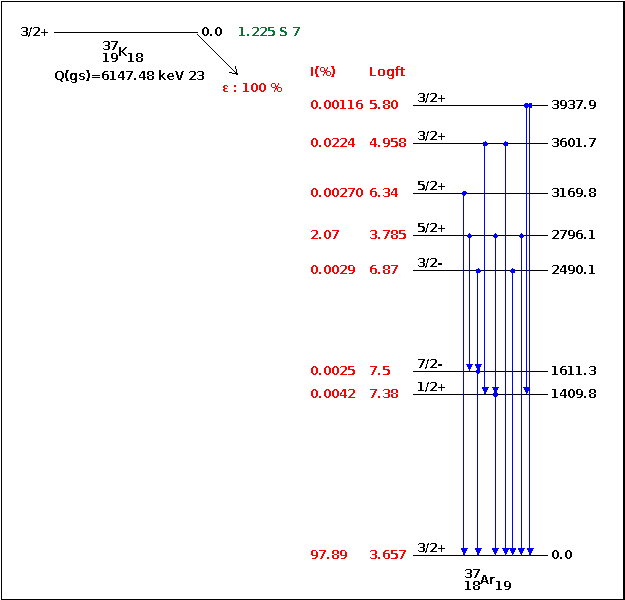
\includegraphics[width=.999\linewidth]{Figures/decayscheme_nndc.png}
	\note[orange, nolist]{Authors: John Cameron, Jun Chen and Balraj Singh, Ninel Nica.
	\\
	Citation:Nuclear Data Sheets 113, 365 (2012) \cite{nucleardata2012}.
	\\...\\
	Also, it's generated by the page from:  National Nuclear Data Center (NNDC) at Brookhaven National Laboratory.  Possibly from the NuDat3 database.
%	https://www.nndc.bnl.gov/nudat3/decaysearchdirect.jsp?nuc=37K&unc=NDS
	}
	\note{Image needs:  title, labels on $I^\pi$ columns, label "energy" on the RH column (which kind of energy?  It's the "level energy".  
	\\
	Also:  describe what "I(\%)" is, or maybe just re-do the label.
	}
	\note[jbn]{
	The caption should include that [...] log\_10(fT) [is] a measure of the absolute decay rate (ref. Krane e.g.) \cite{krane}.
the [...] column [that] has $I^\pi$ where I is spin and $\pi$ is parity [should get a label]. This should not only include Dan's thesis for a reference, but the most recent paper with the branches-- it should work to reference P.D. Shidling
et al. Phys Rev C 98 015502 (2018) \cite{shidling2018} which re-did the half-life and summarized the fT value extraction. I see no publication of your branching ratio work, so I referenced Ozmetin's DNP talk in an earlier note. \cite{ozmetin2020}
}
	\caption[New 37K decay scheme]{A newer, better, less generated-by-Dan level diagram for the decay of $\isotope[37]{K}$.  \cite{nucleardata2012} \cite{ChinPhysC2012}. (probably only use the first citation?) }	
	\label{fig:nuclearleveldiagram_new}
	\label{fig:nuclearleveldiagram}
\end{figure}
\FloatBarrier


As in any decay, the angular correlations between the emerging daughter particles provide a rich source of information about the type of interaction that produced the decay.  
This particular decay involves a set of `mirror' nuclei, meaning that the nuclear wavefunctions of the parent and daughter are identical up to their isospin quantum number and corresponding electrical charge.~\aside[jbn]{no one will let you publish air quotes, ever. Have mercy on your committee, take them all out.  Use the opportunity to make sure you've defined them.
\\...\\
Here, just say isobaric mirror nuclei. You define it right there in text. It's fine to use textbook terms as long as you define them immediately.} \noindent
Because the two wavefunctions are so similar, effects to the decay from nuclear structure corrections can be kept to a minimum, and it is therefore possible to place especially strong constraints on the size of the theoretical uncertainties associated with the decay.  \aside[bluetodo]{Is it definitely true that the nuclear structure corrections are *smaller*?  Or is it just that they're better understood?}


%As a result, observations of this particular decay can be used to place especially strong constraints on 
%This property allows us to place strong constraints on the size of the theoretical uncertainties for this decay process within the Standard Model.  

%\note{ ``Of particular interest is the decay process: $^{37}\textrm{K} \rightarrow \,^{37}\textrm{\!Ar} + \beta^{+} + \nu_e$.  Among other useful properties, this is is a `mirror' decay, meaning that the nuclear wavefunctions of the parent and daughter are identical up to their isospin quantum number.  
%%the number of protons in the parent nucleus (19) is equal to the number of neutrons in the daughter, and the number of neutrons in the parent (18) is equal to the number of protons in the daughter.  
%This property allows us to place strong constraints on the size of the theoretical uncertainties for this decay process within the Standard Model.   %We further exploit this property by noting that both the $^{37}\textrm{K}$ parent and the $^{37}\textrm{\!Ar}$ daughter have nuclear spin $I=3/2$, a fact which is key to this experiment.
%''}


%\note{Talk about how great \isotope[37]{K} is for what we're doing with it.  Also, drop all the math-numbers to support those assertions.  Reference the level diagram within the text!}

\note{Also, 37K is a really nice isotope for this, because 
%98\% + 2\%, 
%also because it's a mirror decay, 
%also because it's an alkali.  Also-
%also, 
its big $\Abeta$ value means we have a big thing to multiply any $\bFierz$ value there might be when we construct the superratio asymmetry to eliminate systematics.}

%\missingfigure{This thing is going to need a nuclear level diagram for 37K.  Also, 37K is a really nice isotope for this, because 98\% + 2\%, also because it's a mirror decay, also because it's an alkali.  Also-also, its big $\Abeta$ value means we have a big thing to multiply any $\bFierz$ value there might be when we construct the superratio asymmetry to eliminate systematics.}


%\section{Exotic Couplings}
%%	In particular, we're interested in so-called scalar and tensor couplings within the nuclear weak force. Standard model beta decay involves only vector and axial-vector couplings, combined with a ``$(V-A)$'' handedness (left-handed).  



%%%% --- * --- %%%%	
\section{The Shake-off Electron Spectrum}
\label{section:soe_intro}
Although the beta decay process is primarily concerned with the emission of beta particles (electrons or positrons) from a Weak interaction that occurs within the nucleus, it is common for one or more \emph{orbital} electrons to also be lost in the process.  Although beta particles are emitted over a continuous energy spectrum, they commonly carry several MeV of kinetic energy.  By contrast, an atomic electron that becomes unbound in this process is likely to only carry a few eV of kinetic energy, and we say that they are `shaken' off.  
\note[jbn]{These are referred to as shakeoff electrons (SOEs), since they are in some sense shaken off.}

We will amend Eq.~\ref{eq:ourdecay} to reflect the presence of $N$ such `shake-off electrons' (SOEs) within each decay event, as
\bea
^{37}\textrm{K} &\rightarrow& \,^{37}\textrm{\!Ar}^{(N-1)+} + \beta^{+} + \nu_e + N \, e_{\textrm{SO}}, 
\label{eq:ourdecay_withsoe}
\eea
%\aside{Do I want to re-assign N somehow so the notation works better?}
where it is clear that, since the parent $^{37}\textrm{K}$ atom was electrically neutral before its decay by $\beta^+$ emission, the daughter $^{37}\textrm{\!Ar}$ will initially have an `extra'~\aside[jbn]{'extra' -> extra. You're not breaking charge conservation here, you don't need to define the word.} orbital electron (and therefore a negative net charge) if no electrons are shaken off.  We also note that it is common for multiple SOEs to be created in a given decay event.  

A further consideration is that the outer electron in an $^{37}\textrm{\!Ar}^{-}$ ion is \emph{not bound},~\aside{cite someone!!  I don't know who.} and in an electric field such as is present within our experimental chamber, this outer electron is removed immediately to be accelerated through the field, leaving behind a neutral $^{37}\textrm{\!Ar}$ atom.  Although this is in principle a different physical loss mechanism, we will refer to unbound electrons resulting from either process as SOEs.  

It is useful to consider the energy spectrum of these shake-off electrons.  The most straightforward component of the SOE energy spectrum arises from the electrons that are lost immediately following decay, and we take these to initially have 0eV in kinetic energy.  

For the shake-off electrons arising from the Weak process itself, the initial energy spectra for SOEs originating in a particular orbital shell can be estimated according to the procedure outlined by Levinger, who credits Feynman for the suggestion~\cite{Levinger}.
~\note[done, nolist]{JB:  \\
$\rightarrow$``by Levinger, who credits Feynman for the suggestion~\cite{Levinger}.''
\\...\\
(Since this is a true story that is not embellished by Feynman in someone else's joke book, but is in a footnote in the Physical Review,  I like to mention it.)
}  \noindent
The strategy is to assume that the sudden approximation holds, and simply calculate the overlap in electron wavefunctions between the initial and final states, where the final state may be either an outgoing electron or one bound within the atom.  Analytic expressions can be obtained if the atom is treated as being hydrogenic -- an excellent approximation here, as $^{37}\textrm{K}$ is an alkali.  

Unfortunately, this treatment cannot determine the fractional contribution of each orbital to the total, nor can it determine the \emph{number} of electrons likely to be removed in a single decay event.  The implications of the SOE energy spectrum to the present experiment are discussed further in Section~\ref{sec:tof_bg}.

\note[bluetodo]{In the end, we used $(0.09)*(\textrm{0eV}) + (0.91)*(0.85*(\textrm{4S}) + 0.15*(\textrm{3P}))$.  But I say that in the other section.  Also, John used Eq.20 for the 4S, and Eq.24 for the 3P.}
\note{Comment on how well this matches our data?  Somehow?}

%\note{Should I talk about the distribution of how many SOEs come off in a decay?  I have measurements of the recoil charge distribution, which is related but not really the same thing.  From a theoretical POV, I don't know how many get shaken off.  Thankfully, it doesn't matter very much in the end.}

%%%%%\begin{figure}[h!!t]
%%%%%	\centering
%%%%%	\includegraphics[width=.999\linewidth]
%%%%%	{Figures/Levinger_SOETOF_prelim.pdf}
%%%%%	\note[clean]{Clean up SOE TOF pic in intro.  It doesn't show what I need!}
\note{A picture of the SOE spectrum for the intro was here.  It's gone now, but it's important that we remember!}
%%%%%	\note{Maybe just kill this picture?  At least reference it in the text somewhere.}
%%%%%	\caption[Levinger TOF]{Shake-off electron TOF (w.r.t. beta TOA) spectrum, showing how the spectrum is different if one includes different sets of initial electrons to be shaken off.  I forget why some of them have 0 eV.  Maybe those are the ones from the $\isotope[37]{Ar}^+$. ... Levinger TOF spectra for some different sets of SOE initial orbitals before shake-off.  (At least that's what it's supposed to be, after I fix the picture).  It's reconstructed event-by-event with beta times-of-flight that would pass some basic `good event' cuts.  Anyway, it turns out, it doesn't much matter what orbitals you lose SOEs from.  That's nice.  In the end, I used 85+15.  \comment{(Need to re-plot this.)} }	
%%%%%	\label{fig:levinger_TOF}
%%%%%\end{figure}


%%%% --- * --- %%%%
\FloatBarrier  % This will have to go away later.
\section{Fierz Interference -- The Physical Signature}
\label{signature_chapter}
\note[orange]{Prototype abstract blurb on the superratio:
\\...\\
While the \emph{overall} size of the effect does not vary as a function of beta emission angle relative to the nuclear spin polarization, other effects do, and so the \emph{fractional} size of the effect also changes.  By constructing the superratio asymmetry, this feature allows for the cancellation of many systematic effects, at the cost of some statistical power.  
}

The physical effects resulting from the presence of scalar or tensor couplings include a small perturbation to the energy spectrum of betas produced by radioactive decay, labeled $\bFierz$ in Eq.~\ref{equation:integrated_jtw}.  Within the Standard Model, the parameter $\bFierz$ is identically zero, and a departure from that would be indicative of (BSM) scalar or tensor couplings.  

The measured value of $\bFierz$ can be evaluated by using a simple beta energy spectrum, as in the top plot of Fig.~\ref{fig:FierzSignature}, but by~\aside[jbn]{$\rightarrow$ not only by.... but also by...} constructing a so-called ``superratio asymmetry'' instead (bottom plot in Fig.~\ref{fig:FierzSignature}), these small changes to the overall spectrum are amplified, and many systematic effects cancel out entirely.  This result comes at the cost of an increased statistical uncertainty.
\note[jbn]{By normalizing Eq.~\ref{equation:integrated_jtw_INTRODUCTION} to have a conventional angular distribution 1 + (term)*$\Abeta$, we can write 
$W(\theta) = 1 + \Abeta/(1+\bFierz \E/\me) cos(\theta) 
\approx 
1 + \Abeta cos(\theta) - \bFierz \E/\me \Abeta cos(\theta) $
for small $\bFierz$.
Our  superratio observable measures directly the coefficient of the $cos(\theta)$ term., and its distortion with energy is multiplied by $\bFierz \Abeta$.
\\...\\
The 37K $\Abeta$ is much larger than the neutron's $\Abeta$, so we gain in sensitivity compared to the neutron.
}
\begin{figure}[h!!t]
	\centering
	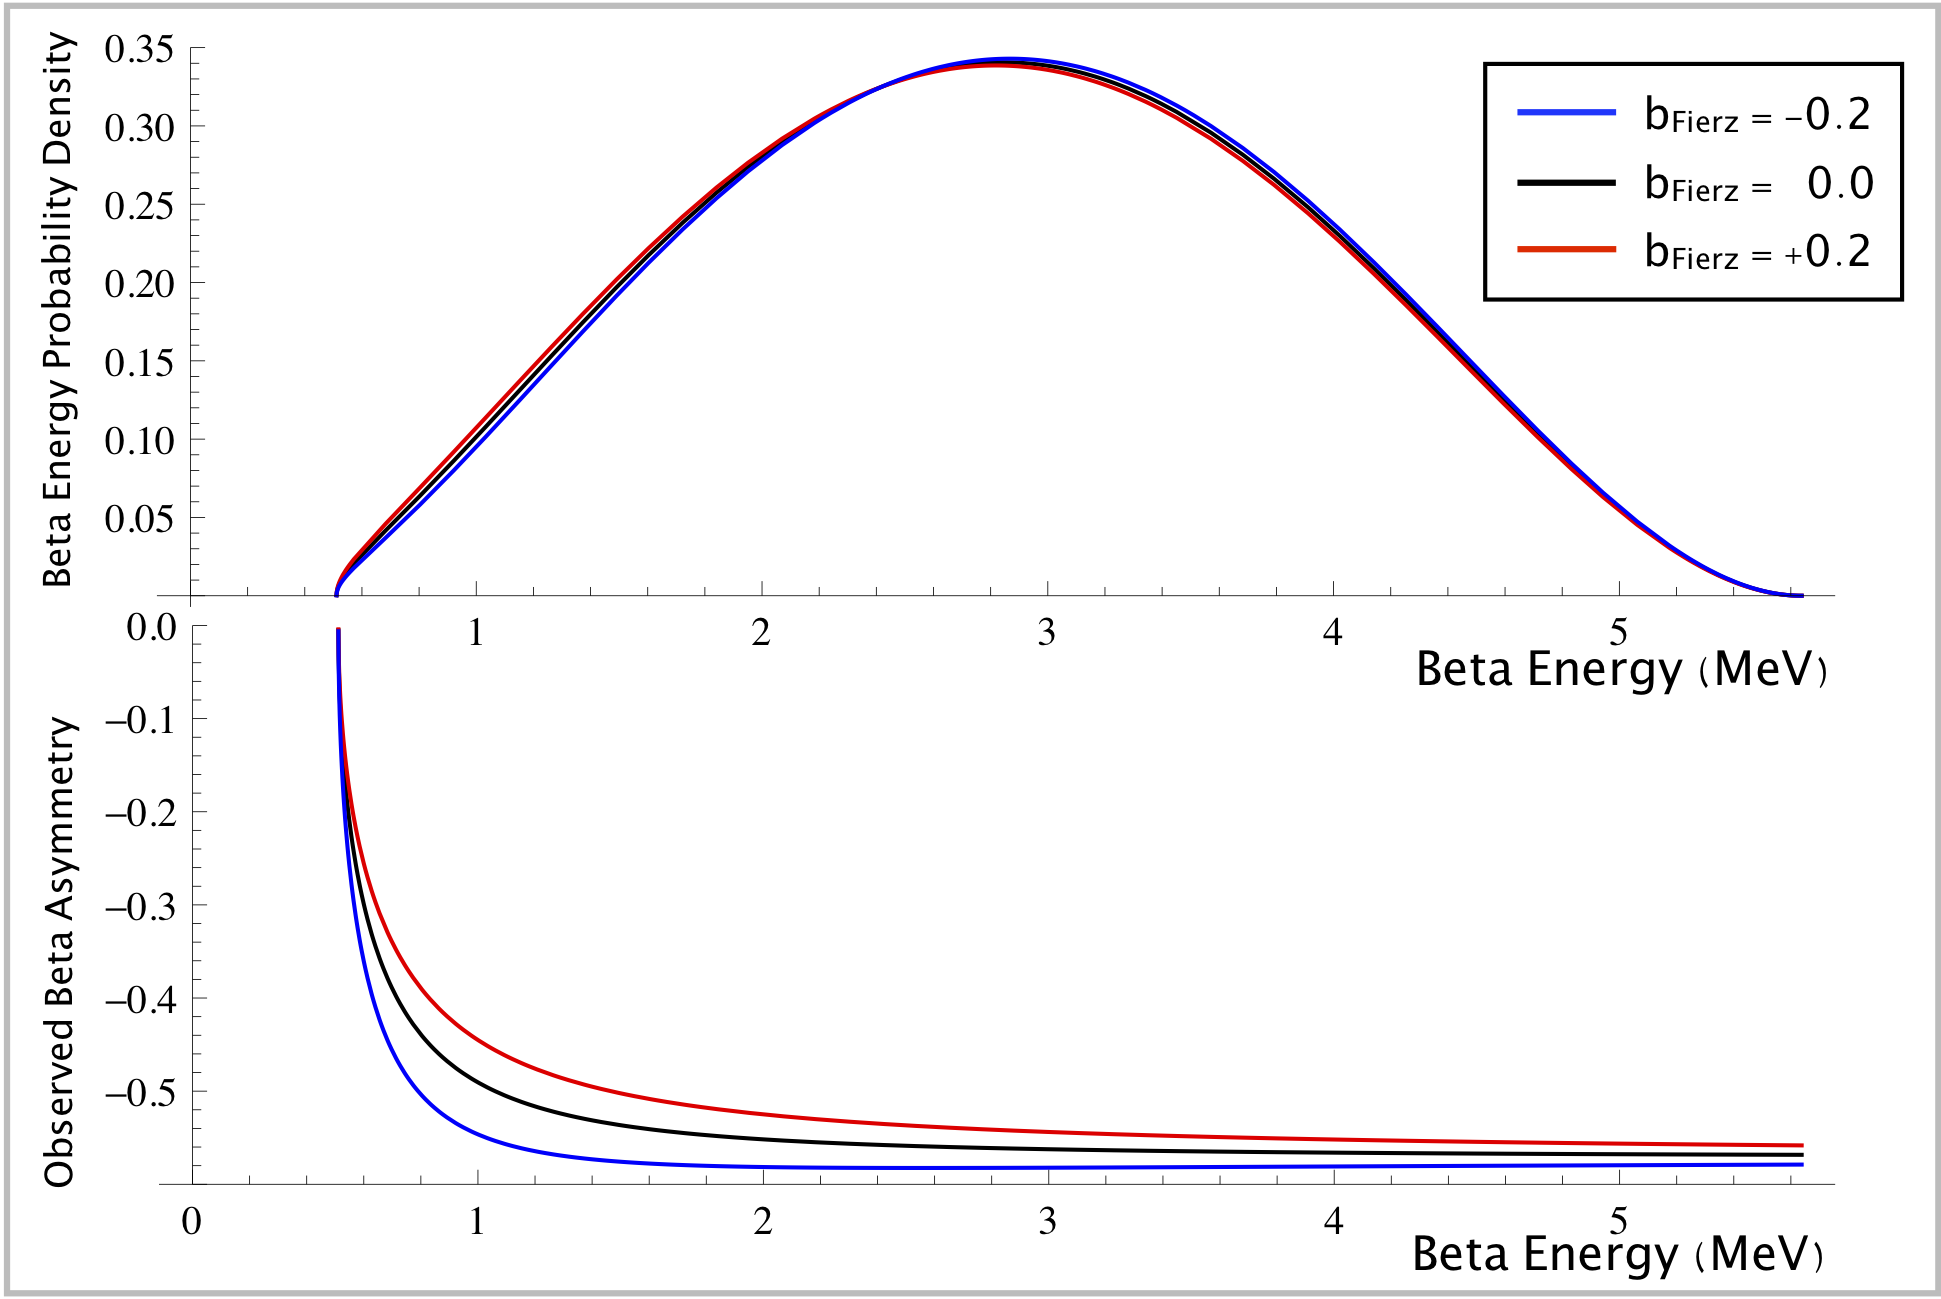
\includegraphics[width=.999\linewidth]
	{Figures/Fierz_Signature.png}
	\caption[Naive Beta Energy Spectrum and Superratio Asymmetry to Measure $\bFierz$]{A naive beta energy spectrum (top) and superratio asymmetry (bottom) are constructed to measure $\bFierz$.}	
	\label{fig:FierzSignature}
\end{figure}

The superratio and superratio asymmetry are discussed in detail in Appendix~\ref{appendix:superratio}.  The discussion includes details on which sort of systematic errors will cancel out entirely, or to leading order, with this treatment -- however it must be noted that for this project, higher-order corrections are included in all simulations, and the effects are propagated through to the end of the analysis.  Therefore, measured values of $\Abeta$ (and $\bFierz$, though that is trivial) may be directly compared to theoretical predictions.  

%%%, and the sort of systematic errors that cancel out under this treatment are discussed in detail in Appendix~\ref{appendix:superratio}.


\note{the "Physical Signature" section probably needs more work, but it's not getting it tonight.}
\note[jb1]{JB on simple things still missing:
\\
Intro or theory section:
\\...\\
P(cos(theta)) = 1 + bm/E + P  Abeta v/c cos(theta)
\\
where theta is the angle between beta and polarization direction
\\...\\
Higher-order corrections to this equation (citing your appendices and/or
chapters) are included in the simulation,
so you are extracting b and Abeta in this
equation to be compared with theory
\\...\\
\{This is a simple but vital statement-- some people actually extract Abeta(Ebeta$=$0) without recoil-order corrections, which is not the same parameter.\}
\\...\\
The theory prediction for Abeta (citing Fenker PRL) is X.
\\
The theory prediction for bFierz is 0 (maybe you have that already).
}

%\note[jb1]{JB:  ``I doubt I will have further useful comments on the Ch. (((this chapter))) as they are now.'' }

%\missingfigure{I need that simulated picture of the different beta energy spectra, with different values of $\bFierz$.}
\note[jb1]{JB on that missing figure that I've now put in:    ``A dependence of Abeta on beta energy is also introduced.
\\
UCNA fits energy spectrum and Abeta[Ebeta] simultaneously now."
}

%\section{Present Limits}
%	A bit about other people's physics.

\note{The point is, the presence of either scalar or tensor interactions will produce a $\bFierz$ term in the decay PDF.  It has other effects on the PDF, but those come in at higher-order in the tiny scalar and tensor couplings.  So, the Fierz term would be by far the biggest thing that changes in the PDF.  The PDF describes the energy and momentum of the outgoing beta w.r.t. a variety of other things.  Notably, we can write an elegant-ish description of beta momentum w.r.t. nuclear polarization direction, and ignore the neutrino completely after integrating over it.  We have a PDF in beta \emph{direction} (w.r.t. polarization), and beta \emph{energy}.  To lowest order (and lowest order is best order) the distribution w.r.t. polarization direction doesn't change, but the distribution w.r.t. energy does change.  Or ... something?  The point is, it makes a change in the beta energy spectrum.  This change is most pronounced at low energies, because the Fierz term is scaled by $(1/\Ebeta)$.  However, the asymmetry is also a function of $\Ebeta$.  A different function of $\Ebeta$.  In fact, it is scaled by $(\pbeta/\Ebeta)$ within the PDF, which is distinctly different than $\bFierz$.  So, one might ask what effect a $\bFierz$ term would produce on a constructed asymmetry spectrum.  ....This explanation has gone way off track.}

\note{Here's a reference to the picture that shows the result of a non-zero $\bFierz$ term.  It's Fig.~\ref{fig:FierzSignature}.}



\note{Kludge-deleted section:  ``On the Superratio, the Supersum, and the Constructed Asymmetry''}
%\section{On the Superratio, the Supersum, and the Constructed Asymmetry}
\note{Clean Superratio,Supersum,Super-Asymmetry section.  Prolly merge w/ bFierz section.}
\note[jb1]{JB:  You need to at some point say that the supersum is the beta energy spectrum.  There are experiments trying to do this method better, but they are very difficult.  UCNA published a combined energy spectrum and Abeta[Ebeta] analysis on the neutron in March 2020~\cite{NeutronbFierz_March2020}.
\\...\\
MJA:  I can't help but also notice the follow-up article from September 2020~\cite{Saul2020}.  Ugh. 
}

%\\*
The data can be combined into a superratio asymmetry.  This has the benefit of causing many systematics to cancel themselves out at leading order.  It also will increase the fractional size of the effects we're looking for.  This can be shown by using math.~\aside[jbn]{``This is shown in full detail in Appendix~\ref{appendix:superratio}.''}

%\\*
Not all systematics effects are eliminated.  We'll want to be careful to propagate through any effects that are relevant.  Using the superratio asymmetry as our physical observable makes this process a bit messier for the things that don't cancel out, but it's all just math.
~\aside[jbn]{You really need a literature reference to the superratio method here. I know you have one. Danny gave us one a long time ago.
}
Some other groups have performed similar measurements using the supersum as the physical observable.  There are pros and cons to both methods.  I can show, using a back-of-the-envelope calculation, that for this particular dataset, the superratio asymmetry method produces a better result.  
\note[jbn]{If you're not going to do this back-of-envelope calculation here, you need to just reference Appendix D and likely eliminate this paragraph?}

